\documentclass[twoside,10pt]{book}
\usepackage[amsbb,mtpfrak,zswash,mtpcal]{mtpro2}
\usepackage[no-math,cm-default]{fontspec}
\usepackage{xunicode}
\usepackage{xgreek}
\defaultfontfeatures{Mapping=tex-text,Scale=MatchLowercase}
\setmainfont[Mapping=tex-text,Numbers=Lining,Scale=1.0,BoldFont={Minion Pro Bold}]{Minion Pro}
\defaultfontfeatures{Ligatures=TeX}
\font\kefalaio="Minion Pro Bold" at 36pt
\font\ArKef="Minion Pro Bold Italic" at 72pt
\font\OnKef="Times New Roman" at 30pt
\font\OnPar="Minion Pro Bold" at 18pt
\font\mymathL = "MyMathSymbols" at 16pt
\font\mymath = "MyMathSymbols"
\newfontfamily\tnr{Times New Roman}
\usepackage{amsmath}
\usepackage[amsbb,mtpfrak,zswash,mtpcal]{mtpro2}
\usepackage[inner=2.00cm, outer=1.50cm, top=3.00cm, bottom=2.00cm,paperwidth=17cm,paperheight=24cm]{geometry}
\usepackage{makeidx}
\usepackage{longtable,mathimatika,varwidth,ifthen}
\usepackage{etoolbox}
\def\xrwma{red!70!black}
\def\xrwmath{red!80!black}
\makeatletter
\newif\ifLT@nocaption
\preto\longtable{\LT@nocaptiontrue}
\appto\endlongtable{%
\ifLT@nocaption
\addtocounter{table}{\m@ne}%
\fi}
\preto\LT@caption{%
\noalign{\global\LT@nocaptionfalse}}
\makeatother
\makeindex
\DeclareRobustCommand{\Algebra}[1]{\index{{\LARGE\bf Άλγεβρα\\}!#1}}
\DeclareRobustCommand{\Gewmetria}[1]{\index{{\LARGE\bf\vspace*{5mm}Γεωμετρία\\}!#1}}
\DeclareRobustCommand{\Analysh}[1]{\index{{\LARGE\bf\vspace*{5mm}Ανάλυση\\}!#1}}
\DeclareRobustCommand{\Statistikh}[1]{\index{{\LARGE\bf\vspace*{5mm}Στατιστική\\}!#1}}
%------ ΕΙΚΟΝΑ ΓΥΡΩ ΑΠΟ ΚΕΙΜΕΝΟ ------------
\newenvironment{WrapText1}[3][r]
{\wrapfigure[#2]{#1}{#3}}
{\endwrapfigure}

\newenvironment{WrapText2}[3][l]
{\wrapfigure[#2]{#1}{#3}}
{\endwrapfigure}
\newcommand{\apodeiksi}{\textcolor{\xrwma}{\textbf{ΑΠΟΔΕΙΞΗ}\\}}{}
\newcommand{\wrapr}[6]{
\begin{minipage}{\linewidth}\mbox{}\\
\vspace{#1}
\begin{WrapText1}{#2}{#3}
\vspace{#4}#5\end{WrapText1}#6
\end{minipage}}

\newcommand{\wrapl}[6]{
\begin{minipage}{\linewidth}\mbox{}\\
\vspace{#1}
\begin{WrapText2}{#2}{#3}
\vspace{#4}#5\end{WrapText2}#6
\end{minipage}}
%-------------------------------------------
%------ ΛΥΜΕΝΑ ΠΑΡΑΔΕΙΓΜΑΤΑ ΤΙΤΛΟΣ ---------
\newcommand{\Lymena}{\begin{center}
\begin{tikzpicture}
\path[left color=red!70!black,right color=red!80!black,middle color=red!80!white] (-7cm,-.6cm) rectangle (6.5cm,.6cm);
\node at (-.25cm,0) {\Large \textcolor{white}{\textbf{ΛΥΜΕΝΑ ΠΑΡΑΔΕΙΓΜΑΤΑ}}};  
\end{tikzpicture}
\end{center}}
%--------------------------------------
%--------- ΑΛΥΤΕΣ ΑΣΚΗΣΕΙΣ ΤΙΤΛΟΣ ----------
\newcommand{\Alyta}{\begin{center}
\begin{tikzpicture}
\path[left color=cyan!70!black,right color=cyan!80!black,middle color=cyan!80!white] (-7cm,-.6cm) rectangle (6.5cm,.6cm);
\node at (-.25cm,0) {\Large \textcolor{white}{\textbf{ΑΣΚΗΣΕΙΣ - ΠΡΟΒΛΗΜΑΤΑ}}};  
\end{tikzpicture}
\end{center}}
%--------------------------------------------
\usetikzlibrary{shadows,calc}
\usepackage{tcolorbox}
\tcbuselibrary{skins,theorems,breakable}
%---------- ΜΕΘΟΔΟΣ --------------
\newcounter{Methodos}[chapter]
\renewcommand{\theMethodos}{\thechapter.\arabic{Methodos}}
\newenvironment{Methodos}[2][\linewidth]
{\refstepcounter{Methodos}
\begin{tcolorbox}[breakable,
enhanced standard,
boxrule=0.7pt,titlerule=-.2pt,drop fuzzy shadow southeast=black!50,
width=\linewidth,
title style={color=white},
overlay unbroken and first={
\path[left color=cyan!70!black,right color=cyan,draw=black]
([yshift=-\pgflinewidth]frame.north west) to ([yshift=-5pt]title.south west)[rounded corners=2pt] -- ([xshift=-#2-15pt,yshift=-5pt]title.south east) to[rounded corners=2pt] ([xshift=-#2,yshift=-\pgflinewidth]frame.north east) -- cycle;
},
fonttitle=\bfseries,
before=\par\medskip\noindent,
after=\par\medskip,
toptitle=3pt,
top=11pt,topsep at break=-5pt,
colback=white,title={\large Μέθοδος \theMethodos} : {\textcolor{black}{\MakeUppercase{#1}}}]}
{\end{tcolorbox}}
%------------------------------------------
\usepackage{amsthm}
\usepackage{tikz,pgfplots}
\usepackage{tkz-euclide,tkz-fct}
\usepackage{wrapfig}
\usetkzobj{all}
\usepackage{calc}
\usepackage{cleveref}
\usepackage[colorlinks=false, pdfborder={0 0 0}]{hyperref}
\usepackage[framemethod=TikZ]{mdframed}
\newcommand{\ypogrammisi}[1]{\underline{\smash{#1}}}
\usetikzlibrary{backgrounds}
\renewcommand{\thepart}{\arabic{part}}
\definecolor{steelblue}{cmyk}{.7,.278,0,.294}
\definecolor{doc}{cmyk}{1,0.455,0,0.569}
\definecolor{thewrhma}{cmyk}{0,.84,1,0.15}
\usepackage{capt-of}
\usepackage{titletoc}
\usepackage[explicit]{titlesec}
\usepackage{graphicx}
\usepackage{multicol}
\usepackage{multirow}
\usepackage{enumitem}
\usepackage{tabularx}
\usepackage[decimalsymbol=comma]{siunitx}
\tikzset{>=latex}
\makeatletter
\pretocmd{\@part}{\gdef\parttitle{#1}}{}{}
\pretocmd{\@spart}{\gdef\parttitle{#1}}{}{}
\makeatother
\usepackage[titletoc]{appendix}
\usepackage{fancyhdr}
\pagestyle{fancy}
\fancyheadoffset{0cm}
\renewcommand{\headrulewidth}{\iftopfloat{0pt}{.5pt}}
\renewcommand{\chaptermark}[1]{\markboth{#1}{}}
\renewcommand{\sectionmark}[1]{\markright{\it\thesection\ #1}}
\fancyhf{}
\fancyhead[LE]{\thepage\ $\cdot$\ \scshape\nouppercase{\leftmark}}
\fancyhead[RO]{\nouppercase{\rightmark} $\cdot$\ \thepage}
\fancypagestyle{plain}{%
\fancyhead{} %
\renewcommand{\headrulewidth}{0pt}}

\newcounter{thewrhma}[chapter]
\renewcommand{\thethewrhma}{\thechapter.\arabic{thewrhma}}   

\newcommand{\Thewrhma}[1]{\refstepcounter{thewrhma}\textcolor{thewrhma}{\large{\textbf{Θεώρημα\hspace{2mm}\thethewrhma\hspace{1mm}}}} \MakeUppercase{\textbf{#1}}\\}{}

\newcounter{porisma}[chapter]
\renewcommand{\theporisma}{\thechapter.\arabic{porisma}}\newcommand{\Porisma}[1]{\refstepcounter{porisma}\textcolor{black}{\textbf{ΠΟΡΙΣΜΑ\hspace{2mm}\theporisma\hspace{1mm} \MakeUppercase{#1}}}\\}{}

\newcounter{protasi}[chapter]
\renewcommand{\theprotasi}{\thechapter.\arabic{protasi}}\newcommand{\Protasi}[1]{\refstepcounter{protasi}\textcolor{black}{\textbf{ΠΡΟΤΑΣΗ\hspace{2mm}\theprotasi\hspace{1mm} \MakeUppercase{#1}}}\\}{}

\newcounter{methodologia}[chapter]
\renewcommand{\themethodologia}{\thechapter.\arabic{methodologia}}\newcommand{\Methodologia}[1]{\refstepcounter{methodologia}\textcolor{black}{\textbf{MΕΘΟΔΟΣ\hspace{2mm}\themethodologia\hspace{1mm} \MakeUppercase{#1}}}\\}{}

\newcounter{orismos}[chapter]
\renewcommand{\theorismos}{\thechapter.\arabic{orismos}}   
\newcommand{\Orismos}[1]{\refstepcounter{orismos}\textcolor{red!80!black}{\large{\textbf{Ορισμός\hspace{2mm}\theorismos\hspace{1mm}}}} \MakeUppercase{\textbf{#1}}\\}{}
\usepackage{venndiagram}
%-------- ΣΤΥΛ ΚΕΦΑΛΑΙΟΥ ---------
\newcommand*\chapterlabel{}
\newcommand{\fancychapter}{%
\titleformat{\chapter}
{
\normalfont\Huge}
{\gdef\chapterlabel{\thechapter\ }}{0pt}
{\begin{tikzpicture}[remember picture,overlay]
\node[yshift=-7cm] at (current page.north west)
{\begin{tikzpicture}[remember picture, overlay]
%\node[inner sep=0pt] at ($(current page.north) +			(0cm,-1.38in)$) {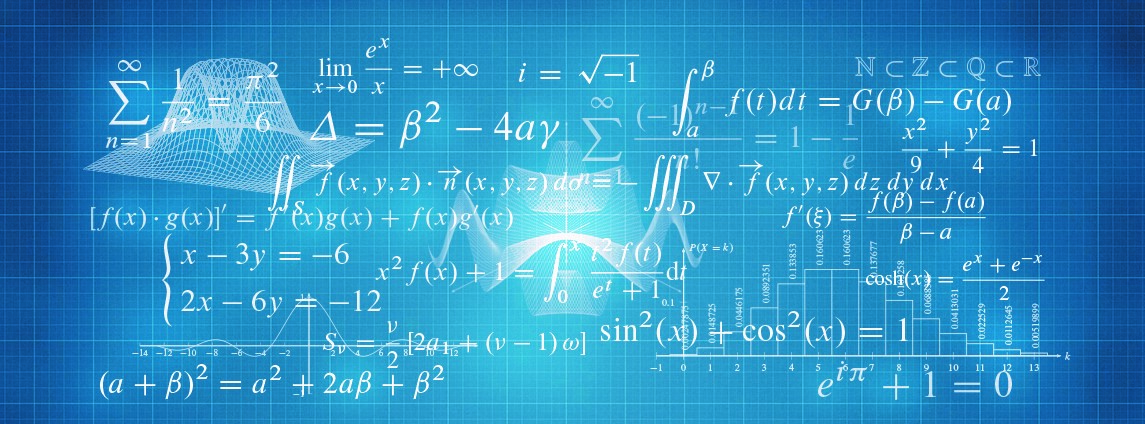
\includegraphics[width=17cm]{Kefalaio}};
\node[anchor=west,xshift=.12\paperwidth,yshift=.17\paperheight,rectangle]
{{\color{white}\fontsize{30}{20}\textbf{\textcolor{black}{\contour{white}{ΚΕΦΑΛΑΙΟ}}}}};
\node[anchor=west,xshift=.11\paperwidth,yshift=.11\paperheight,rectangle] {\fontsize{27}{20} {\color{black}{{\textcolor{black}{\contour{white}{\sc##1}}}}}};
%\fill[fill=black] (12.2,2) rectangle (14.8,4.7);
\node[anchor=west,xshift=.74\paperwidth,yshift=.14\paperheight,rectangle]
{{\color{white}\fontsize{80}{20}\textbf{\textit{\textcolor{white}{\contour{black}{\thechapter}}}}}};
\end{tikzpicture}
};
\end{tikzpicture}
}
\titlespacing*{\chapter}{0pt}{20pt}{30pt}
}
%------------------------------------------------


\usepackage[outline]{contour}
\newcommand{\regularchapter}{%
\titleformat{\chapter}[display]
{\normalfont\huge\bfseries}{\chaptertitlename\ \thechapter}{20pt}{\Huge##1}
\titlespacing*{\chapter}
{0pt}{-20pt}{40pt}
}

\apptocmd{\mainmatter}{\fancychapter}{}{}
\apptocmd{\backmatter}{\regularchapter}{}{}
\apptocmd{\frontmatter}{\regularchapter}{}{}

\titlespacing*{\section}
{0pt}{30pt}{0pt}
\usepackage{booktabs}
\usepackage{hhline}
\DeclareRobustCommand{\perthousand}{%
\ifmmode
\text{\textperthousand}%
\else
\textperthousand
\fi}

\newcounter{typos}[chapter]
\renewcommand{\thetypos}{T\arabic{typos}}   
\newcommand{\Typos}{\refstepcounter{typos}\textcolor{gray}{\textbf{\thetypos}}}{}


\contentsmargin{0cm}
\titlecontents{part}[-1pc]
{\addvspace{10pt}%
\bf\Large ΜΕΡΟΣ\quad }%
{}
{}
{\;\dotfill\;\normalsize\ Σελίδα}%
%------------------------------------------
\titlecontents{chapter}[0pc]
{\addvspace{30pt}%
\begin{tikzpicture}[remember picture, overlay]%
\draw[fill=black,draw=black] (-.3,.5) rectangle (3.7,1.1); %
\pgftext[left,x=0cm,y=0.75cm]{\color{white}\sc\Large\bfseries Κεφάλαιο\ \thecontentslabel};%
\end{tikzpicture}\large\sc}%
{}
{}
{\hspace*{-2.3em}\hfill\normalsize Σελίδα \thecontentspage}%
\titlecontents{section}[2.4pc]
{\addvspace{1pt}}
{\contentslabel[\thecontentslabel]{2pc}}
{}
{\;\dotfill\;\small \thecontentspage}
[]
\titlecontents*{subsection}[4pc]
{\addvspace{-1pt}\small}
{}
{}
{\ --- \small\thecontentspage}
[ \textbullet\ ][]

\makeatletter
\renewcommand{\tableofcontents}{%
\chapter*{%
\vspace*{-20\p@}%
\begin{tikzpicture}[remember picture, overlay]%
\pgftext[right,x=12cm,y=0.2cm]{\Huge\sc\bfseries \contentsname};%
\draw[fill=black,draw=black] (9.5,-.75) rectangle (12.5,1);%
\clip (9.5,-.75) rectangle (15,1);
\pgftext[right,x=12cm,y=0.2cm]{\color{white}\Huge\bfseries \contentsname};%
\end{tikzpicture}}%
\@starttoc{toc}}
\makeatother

\usepackage[contents={},scale=1,opacity=1,color=black,angle=0]{background}

\newcommand\blfootnote[1]{%
\begingroup
\renewcommand\thefootnote{}\footnote{#1}%
\addtocounter{footnote}{-1}%
\endgroup
}
\usepackage{epstopdf}
\epstopdfsetup{update}
\usepackage{textcomp}
\titleformat{\section}
{\normalfont\Large\bf}%
{}{0em}%
{{\color{black}\titlerule[1pt]}\vskip-.2\baselineskip{\parbox[t]{\dimexpr\textwidth-2\fboxsep\relax}{\raggedright\strut\thesection~#1\strut}}}[\vskip 0\baselineskip{\color{black}\titlerule[1pt]}]
\titlespacing*{\section}{0pt}{0pt}{0pt}

\newcommand{\methodologia}{\begin{center}
{\large \textbf{ΜΕΘΟΔΟΛΟΓΙΑ}}\\\vspace{-2mm}
\begin{tikzpicture}
\shade[left color=white, right color=black] (-3cm,0) rectangle (0,.2mm);
\shade[left color=black, right color=white] (0,0) rectangle (3cm,.2mm);   
\end{tikzpicture}
\end{center}}

\newcommand{\orismoi}{\begin{center}
\large \textbf{ΟΡΙΣΜΟΙ}\\\vspace{-2mm}
\begin{tikzpicture}
\shade[left color=white, right color=black] (-3cm,0) rectangle (0,.2mm);
\shade[left color=black, right color=white] (0,0) rectangle (3cm,.2mm);   
\end{tikzpicture}
\end{center}}

%------- ΣΤΥΛ ΠΑΡΑΔΕΙΓΜΑΤΟΣ -------
\newcounter{paradeigma}[section]
\renewcommand{\theparadeigma}{\bf\arabic{paradeigma}}   
\newcommand{\Paradeigma}[1]{\refstepcounter{paradeigma}\textcolor{black}{\textbf{\textcolor{\xrwma}{ΠΑΡΑΔΕΙΓΜΑ\hspace{2mm}\theparadeigma\;:}\;\hspace{1mm}}} \MakeUppercase{\textbf{#1}}\\}{}

\newcommand{\thewrhmata}{\begin{center}
{\large \textbf{ΘΕΩΡΗΜΑΤΑ - ΠΟΡΙΣΜΑΤΑ - ΠΡΟΤΑΣΕΙΣ\\ΚΡΙΤΗΡΙΑ - ΙΔΙΟΤΗΤΕΣ}}\\\vspace{-2mm}
\begin{tikzpicture}
\shade[left color=white, right color=black,] (-3cm,0) rectangle (0,.2mm);
\shade[left color=black, right color=white,] (0,0) rectangle (3cm,.2mm);   
\end{tikzpicture}
\end{center}}
\usepackage[labelfont={footnotesize,it,bf},font={footnotesize}]{caption}
\usepackage{wrapfig}
%-------- ΜΑΘΗΜΑΤΙΚΑ ΕΡΓΑΛΕΙΑ ---------
\usepackage{mathtools,mathimatika}
%----------------------
%-------- ΠΙΝΑΚΕΣ ---------
\usepackage{booktabs}
%----------------------
%----- ΥΠΟΛΟΓΙΣΤΗΣ ----------
%\usepackage{calculator}
%----------------------------

%----- ΟΡΙΖΟΝΤΙΑ ΛΙΣΤΑ ------
\usepackage{xparse}
\newcounter{answers}
\renewcommand\theanswers{\arabic{answers}}
\ExplSyntaxOn
\NewDocumentCommand{\results}{m}
{
\seq_set_split:Nnn \l_results_a_seq {,}{#1}
\par\nobreak\noindent\setcounter{answers}{0}
\seq_map_inline:Nn \l_results_a_seq
{
\makebox[.18\linewidth][l]{\stepcounter{answers}\theanswers.~##1}\hfill
}
\par
}
\seq_new:N \l_results_a_seq
\ExplSyntaxOff

\usepackage{microtype}
\usepackage{float}

\usepackage{caption}
\newcommand{\lysh}{\textbf{\textcolor{\xrwma}{ΛΥΣΗ}}}

%---- ΟΡΙΖΟΝΤΙΟ - ΚΑΤΑΚΟΡΥΦΟ - ΠΛΑΓΙΟ ΑΓΚΙΣΤΡΟ ------
\newcommand{\orag}[3]{\node at (#1)
{$ \overcbrace{\rule{#2mm}{0mm}}^{{\scriptsize #3}} $};}

\newcommand{\kag}[3]{\node at (#1)
{$ \undercbrace{\rule{#2mm}{0mm}}_{{\scriptsize #3}} $};}

\newcommand{\Pag}[4]{\node[rotate=#1] at (#2)
{$ \overcbrace{\rule{#3mm}{0mm}}^{{\rotatebox{-#1}{\scriptsize$#4$}}}$};}
%-----------------------------------------
\newlist{rlist}{enumerate}{3}
\setlist[rlist]{itemsep=0mm,label=\textcolor{\xrwma}{\roman*.}}
\newlist{brlist}{enumerate}{3}
\setlist[brlist]{itemsep=0mm,label=\bf\roman*.}
\newlist{tropos}{enumerate}{3}
\setlist[tropos]{label=\bf\textit{\arabic*\textsuperscript{oς}\;Τρόπος :},leftmargin=0cm,itemindent=1.9cm,ref=\bf{\arabic*\textsuperscript{oς}\;Τρόπος}}
\tikzstyle{pl}=[line width=0.3mm]
\tikzstyle{plm}=[line width=0.4mm]
\tkzSetUpPoint[size=7,fill=white]
\setlength{\parindent}{0pt}
\setlist[itemize]{itemsep=0mm}
\tkzSetUpPoint[size=7,fill=white]
\newcommand{\twocolkentro}[1]{
\twocolumn[
\begin{@twocolumnfalse}
#1
\end{@twocolumnfalse}]}
\newcommand{\bcc}[1]{\begin{center}
\textbf{\textcolor{\xrwma}{#1}}
\end{center}}





\begin{document}
\title{\MakeUppercase{ΣΧΟΛΙΚΟ ΤΥΠΟΛΟΓΙΟ}}
\pagestyle{empty}
\frontmatter
\begin{titlepage}
\newgeometry{left=2.5cm,top=2.5cm} %defines the geometry for the titlepage
\pagecolor{white}
\begin{center}
{\large Σπύρος Φρόνιμος\\Μαθηματικός}
\end{center}
\noindent
\par
\noindent
\mbox{}\\\\
\begin{center}
\textbf{\fontsize{20}{40}\selectfont{ΤΑ ΕΚΤΟΣ ΥΛΗΣ}}\par\mbox{}\\\vspace{-3mm}
\textbf{\fontsize{20}{40}\selectfont{ΓΥΜΝΑΣΙΟΥ - ΛΥΚΕΙΟΥ}}\par\mbox{}\\
\vspace{-4mm}
\rule{12cm}{0.1mm}\\
\vspace{3mm}
{\fontsize{15}{15}\MakeUppercase{Η "ΑΔΙΚΗΜΕΝΗ" ΘΕΩΡΙΑ ΤΩΝ ΜΑΘΗΜΑΤΙΚΩΝ}}\\
\vspace{.7mm}
{\fontsize{15}{15}\MakeUppercase{ΤΩΝ ΣΧΟΛΙΚΩΝ ΒΙΒΛΙΩΝ}}\\
\rule{12cm}{0.1mm}\\
\end{center}
\vspace{3cm}
\begin{flushright}
\begin{itemize}
\item 100 Ορισμοί
\item 250 Θεωρήματα
\item 400 Μέθοδοι για λύση ασκήσεων
\item 200 Λυμένα παραδείγματα
\item 500 Άλυτες ασκήσεις και προβλήματα
\item 200 Επαναληπτικά θέματα
\item Απαντήσεις ασκήσεων
\end{itemize}
\end{flushright}

\vfill
\noindent
\color{black}
\begin{center}
{\large{ΕΚΔΟΣΕΙΣ \_\_\_\_\_}\\
\large{ΚΕΡΚΥΡΑ 2015}}
\vskip\baselineskip
\end{center}
\hbox{ % Horizontal box
\hspace*{0.2\textwidth} % Whitespace to the left of the title page
\rule{1pt}{\textheight} % Vertical line
\hspace*{0.05\textwidth} % Whitespace between the vertical line and title page text
\parbox[b]{0.75\textwidth}{ % Paragraph box which restricts text to less than the width of the page

{\textbf{Αλγεβρα}\\\textbf{Β΄ Λύκείου}\\\\\noindent \textbf{Σπύρος Φρόνιμος - Μαθηματικός}\\e-mail : spyrosfronimos@gmail.com\\[0.5\baselineskip]
Σελίδες : ...\\
ΙΣΒΝ : ...\\
Εκδόσεις : ...\\
\textcopyright Copyright 2015}\\[2\baselineskip] % Title
{Φιλολογική Επιμέλεια :\\\textbf{Μαρία Πρεντουλή}}
{- e-mail : predouli@yahoo.com}\\[0.5\baselineskip]
{Επιστημονική Επιμέλεια :}{\textbf{Σπύρος Φρόνιμος}}\\[0.5\baselineskip]
{Εξώφυλλο : \\\textbf{Δημήτρης Πρεντουλής}}\\[1\baselineskip] % Tagline or further description
% Author name

\vspace{.4\textheight} % Whitespace between the title block and the publisher
{Πνευματικά Δικαιώματα : ...}\\[\baselineskip]}}
\vspace*{2\baselineskip}
\newpage
\mbox{}\\\\\\\\\\\\
\hspace*{0.75\textwidth}
\textit{{\large Στη γυναίκα μου.}}
\newpage
\mbox{}
\newpage
\mbox{}
{\LARGE \textbf{Πρόλογος}}\\\\\\\\

Το βιβλίο περιέχει συγκεντρωμένη όλη τη θεωρία των μαθηματικών όλων των τάξεων του γυμνασίου και του λυκείου γραμμένη αναλυτικά και κατανοητά.\\\\
Ειδικότερα ο αναγνώστης θα βρει\\
\vspace{-.4cm}
\begin{itemize}
\item Ορισμούς
\item Θεωρήματα
\item Τυπολόγιο
\item Μεθοδολογία
\end{itemize}
Σκοπό έχει να αποτελέσει ένα χρήσιμο βοήθημα για μικρούς ή μεγάλους μαθητές όπου μπορούν να έχουν όλη τη θεωρία της χρονιάς τους συγκεντρωμένη, χρήσιμη για επανάληψη και διαγωνίσματα, αλλά και να μπορούν εύκολα να καλύψουν τυχόν κενά από προηγούμενες τάξεις.\\\\\\
Θέλω να ευχαριστήσω όλους όσους βοήθησαν.
\newpage
\end{titlepage}
\restoregeometry % restores the geometry
\tableofcontents
\mainmatter
\pagestyle{fancy}
\chapter{Άλγεβρα}
\section{Τριγωνομετρικές ανισώσεις}\mbox{}\\
Ανάλογα με τις βασικές τριγωνομετρικές εξισώσεις που συναντήσαμε στην άλγεβρα της Α΄ και Β΄ Λυκείου, μπορούν να οριστούν και οι τριγωνομετρικές ανισώσεις των οποίων οι βασικές μορφές με τις οποίες θα ασχοληθούμε αρχικά είναι 
\[ \hm{x}>a \ (\textrm{ή }<a)\ ,\ \syn{x}>a\ (\textrm{ή }<a)\ ,\ \ef{x}>a\ (\textrm{ή }<a)\ ,\ \syf{x}>a\ (\textrm{ή }<a) \]
Η λύση μιας τριγωνομετρικής ανίσωσης ανάγεται στην εύρεση του κατάλληλου συνόλου γωνιών που την ικανοποιούν. Την επίλυση βοηθάει αρκετά η χρήση του τριγωνομετρικού κύκλου πάνω στον οποίο οι λύσεις, όπως θα δούμε στη συνέχεια, θα παρασταθούν γραφικά ως ένα ή περισσότερα τόξα. Για να απλουστεύσουμε τη διαδικασία εργαζόμαστε αρχικά στο διάστημα ενός κύκλου. Ας δούμε όμως αρχικά τι ονομάζεται τριγωνομετρική ανίσωση.\\\\
\Orismos{Τριγωνομετρική ανίσωση}
Τριγωνομετρική ονομάζεται κάθε ανίσωση η οποία περιέχει τουλάχιστον ένα τριγωνομετρικό αριθμό. Οι βασικές μορφές τριγωνομετρικών ανισώσεων είναι :
\[ \hm{x}>a\ ,\ \syn{x}>a\ ,\ \ef{x}>a\ ,\ \syf{x}>a\ ,\ a\in\mathbb{R} \]
\begin{itemize}
\item Λύση μιας τριγωνομετρικής ανίσωσης ονομάζεται κάθε αριθμός που την επαληθεύει.
\item Το σύνολο των λύσεων σε ένα διάστημα πλάτους μιας περιόδου της αντίστοιχης συνάρτησης ονομάζεται \textbf{ειδική λύση} της ανίσωσης.
\item Το σύνολο όλων των λύσεων της ονομάζεται \textbf{γενική λύση}.
\end{itemize}
Ομοίως ορίζονται οι ανισώσεις με τους συμβολισμούς $ <,\geq,\leq $ μεταξύ του τριγωνομετρικού αριθμού και του πραγματικού αριθμού $ a $.\\\\
Απλά παραδείγματα τέτοιων ανισώσεων όπως $ \hm{x}>\frac{1}{2}\ ,\ \syn{x}\leq\frac{\sqrt{2}}{2}\ ,\ \ef{x}<1\ ,\ \syf{x}\geq0 $ είναι αυτά που θα μας βοηθήσουν να κατανοήσουμε τη διαδικασία επίλυσης για κάθε περίπτωση.
\begin{enumerate}[itemsep=0mm,label=\textcolor{\xrwma}{\bf\arabic*.},leftmargin=0mm,itemindent=4mm]
\item \textbf{\textcolor{\xrwma}{Η ανίσωση {\boldmath$ \hm{x}>a $}}}\\
Ας ξεκινήσουμε με τη μελέτη της ανίσωσης $ \hm{x}>a $.  Όπως και στην επίλυση των εξισώσεων έτσι κι εδώ αναζητούμε την ύπαρξη κατάλληλης γωνίας της οποίας το ημίτονο να ισούται με τον αριθμό $ a $. Για τον πραγματικό αριθμό $ a $ εξετάζουμε τις ακόλουθες περιπτώσεις :
\begin{itemize}
\item Αν $ a\geq1 $ τότε η ανίσωση είναι αδύνατη.
\item Αν $ a<-1 $ τότε η ανίσωση είναι αόριστη.
\item Αν $ a=-1 $ τότε οι λύσεις της ανίσωσης είναι όλες οι γωνίες εκτός από τις λύσεις της εξίσωσης $ \hm{x}=-1 $.
\item Αν $ a\in(-1,1) $ τότε αναζητούμε κατάλληλη γωνία $ \theta $ ώστε $ \hm{\theta}=a $. Διακρίνουμε τις εξής υποπεριπτώσεις.
\end{itemize}
\begin{rlist}[leftmargin=0mm,itemindent=4mm]
\item Αν $ a\in[0,1) $ τότε 
ας υποθέσουμε ότι $ \theta\in\left[0,\frac{\pi}{2}\right)  $ είναι η ζητούμενη γωνία. Τότε η ανίσωση θα γραφτεί
\[ \hm{x}>\hm{\theta} \]
Λύνοντας την αντίστοιχη εξίσωση $ \hm{x}=\hm{\theta} $ στο διάστημα $ [0,2\pi] $ παίρνουμε τις γωνίες $ x=\theta $ και $ x=\pi-\theta $ δηλαδή τις παραπληρωματικές γωνίες. Έτσι οι λύσεις της ανίσωσης θα είναι οι γωνίες που βρίσκονται μεταξύ των παραπληρωματικών αυτών γωνιών και θα δίνονται από τον τύπο
\[ \theta<x<\pi-\theta\Leftrightarrow x\in(\theta,\pi-\theta) \]
\wrapr{-5mm}{7}{4.3cm}{-12mm}{\begin{tikzpicture}[scale=1.2]
\draw(-1.1,.767)--(1.1,.767);
\trigkyklos
\triganiswsh{50}{130}{A}{B}
\node at (-.15,.6){$K$};
\tkzDefPoint[label=$M$](77:1){C}
\tkzLabelPoint[above right](A){$A(\theta)$}
\tkzLabelPoint[above left](B){$B(\pi-\theta)$}
\node at (-1.3,.57){{\footnotesize $ y=a $}};
\draw (0:.3) arc (0:50:.3);
\draw (0:.25) arc (0:77:.25);
\node at (.4,.2){{\footnotesize $ \theta $}};
\draw(C)--(0,0);
\tkzDrawPoint(C)
\end{tikzpicture}}{
Αντιμετωπίζοντας την αρχική ανίσωση γεωμετρικά με τη βοήθεια του τριγωνομετρικού κύκλου σχεδιάζουμε την ευθεία $ y=a $ που διέρχεται από το σημείο $ K(0,a) $ του άξονα των ημιτόνων. Αυτή τέμνει τον τριγωνομετρικό κύκλο στα σημεία $ A,B $ των γωνιών $ \theta,\pi-\theta $ αντίστοιχα.
Τα σημεία του κύκλου με τετμημένη μεγαλύτερη από $ a $ ορίζουν τόξο με άκρα τα σημεία $ A,B $. Το τόξο αυτό βρίσκεται\textbf{ πάνω από την ευθεία} $ y=a $. Επομένως οι λύσεις θα είναι οι γωνίες που ορίζουν τα εσωτερικά σημεία $ M $ του τόξου $ AB $.}
\[ x\hat{O}A<x<x\hat{O}B\Rightarrow \hm\left( x\hat{O}A\right) <\hm{x}<\hm{\left(x\hat{O}B\right)} \]
Γενικεύοντας τα συμπεράσματα αυτά για τα διαστήματα των υπόλοιπων κύκλων παίρνουμε τη γενική λύση της αρχικής ανίσωσης \[ x\in\left(2\kappa\pi+\theta,2\kappa\pi+\left( \pi-\theta\right) \right)\ ,\ \kappa\in\mathbb{Z} \] Το γενικό σύνολο λύσεων προέκυψε προσθέτοντας πολλαπλάσια της περιόδου $ 2\pi $ της συνάρτησης $ f(x)=\hm{x} $ με $ \kappa\in\mathbb{Z} $.
Θα δούμε μια επιπλέον γραφική παράσταση των λύσεων κατασκευάζοντας τη γραφική παράσταση της συνάρτησης $ f(x)=\hm{x} $ με πεδίο ορισμού ένα διάστημα πλάτους τουλάχιστον μιας περιόδου καθώς και τις οριζόντιες ευθείες $ y=a $ και $ y=1 $. Το μέρος της γραφικής παράστασης που βρίσκεται \textbf{μεταξύ των δύο ευθειών} περιέχει σημεία με τετμημένες που πληρούν τη συνθήκη $ \hm{x}>\hm{\theta} $. Οι τετμημένες αυτές είναι οι λύσεις της ανίσωσης.
\begin{center}
\begin{tikzpicture}
\fill[\xrwma!10] (.28,2.24) rectangle (9.1,2.73);
\draw[shift={(2.8mm,3.5mm)},style=help lines, xstep=0.5497cm,ystep=0.297cm,black!20] (0,0) grid (8.796,2.38);
\begin{axis}[x=.7cm,y=.7cm,xtick={
-6.28318, -4.7123889, -3.14159, -1.5708,
1.5708, 3.14159, 4.7123889, 6.28318,7.854,9.424,10.995,12.564},
xticklabels={
$-2\pi$, $-\frac{3\pi}{2}$, $-\pi$, $\frac{\pi}{2}$,
$\frac{\pi}{2}$, $\pi$, $\frac{3\pi}{2}$, $2\pi$,$\frac{5\pi}{2}$,$3\pi$,$\frac{7\pi}{2}$,$4\pi$
},ytick={-1.7,-.85,0.85,1.7},yticklabels={$-1$,$-0.5$,$0.5$,$1$},aks_on,xmin=-.4,xmax=13.2,
ymin=-2.2,ymax=2.2,xlabel={\footnotesize $ x $},
ylabel={\footnotesize $ y $},belh ar,clip=false]
\addplot[samples=200,domain=0:4*pi]{1.7*sin(deg(x))};
\addplot[grafikh parastash,domain=pi/5:4*pi/5]{1.7*sin(deg(x))};
\addplot[grafikh parastash,domain=11*pi/5:14*pi/5]{1.7*sin(deg(x))};
\coordinate (A) at (axis cs:pi/5,1);
\coordinate (B) at (axis cs:4*pi/5,1);
\coordinate (C) at (axis cs:11*pi/5,1);
\coordinate (D) at (axis cs:14*pi/5,1);
\draw (axis cs:-.2,1)--(axis cs:12.7,1);
\draw (axis cs:-.2,1.7)--(axis cs:12.7,1.7);
\draw[plm,\xrwma] (axis cs:pi/5,0)--(axis cs:4*pi/5,0);
\draw[plm,\xrwma] (axis cs:11*pi/5,0)--(axis cs:14*pi/5,0);
\draw[dashed] (axis cs:pi/5,0)node[below=4mm]{\footnotesize$\theta$}--(axis cs:pi/5,1);
\draw[dashed] (axis cs:4*pi/5,0)node[below=4mm]{\footnotesize$\pi-\theta$}--(axis cs:4*pi/5,1);
\draw[dashed] (axis cs:11*pi/5,0)node[below=4mm]{\footnotesize$2\pi+\theta$}--(axis cs:11*pi/5,1);
\draw[dashed] (axis cs:14*pi/5,0)node[below=4mm]{\footnotesize$3\pi-\theta$}--(axis cs:14*pi/5,1);
\draw[-latex] (axis cs:pi/5,-.7)--(axis cs:pi/5,-.1);
\draw[-latex] (axis cs:4*pi/5,-.7)--(axis cs:4*pi/5,-.1);
\draw[-latex] (axis cs:11*pi/5,-.7)--(axis cs:11*pi/5,-.1);
\draw[-latex] (axis cs:14*pi/5,-.7)--(axis cs:14*pi/5,-.1);
\node at (axis cs:13.7,1){\footnotesize$y=\hm\theta$};
\node at (axis cs:13.5,1.68){\footnotesize$y=1$};
\end{axis}
\tkzDrawPoints(A,B,C,D)
\node at (0.0951,1.344) {\footnotesize$O$};
\end{tikzpicture}
\end{center}
\item Έστω τώρα ότι $ a\in(-1,0] $ και $ \theta\in\left[ 0,\frac{\pi}{2}\right)  $ η κατάλληλη γωνία ώστε $ \hm{\theta}=-a $. Τότε η ανίσωση θα γίνει
\[ \hm{x}>\hm{(-\theta)} \]
\wrapr{-5mm}{8}{4.9cm}{-8mm}{\begin{tikzpicture}[scale=1.2]
\draw(-1.1,-.767)--(1.1,-.767);
\trigkyklos
\triganiswsh{-50}{230}{A}{B}
\node at (-.15,-.6){$K$};
\tkzDefPoint[label=$M$](70:1){C}
\tkzLabelPoint[below right](A){$A(2\pi-\theta)$}
\tkzLabelPoint[below left](B){$B(\pi+\theta)$}
\node at (-1.3,-.57){{\footnotesize $ y=a $}};
\draw(C)--(0,0);
\tkzDrawPoint(C)
\end{tikzpicture}}{
Οι λύσεις της αντίστοιχης εξίσωσης θα είναι οι $ \pi+\theta $ και $ 2\pi-\theta $. Επομένως οι λύσεις της ανίσωσης στο διάστημα $ [0,2\pi] $ θα ανήκουν στο σύνολο \[ [0,\pi+\theta)\cup\left(2\pi-\theta,2\pi\right] \] Αυτό μπορεί να φανεί και γραφικά με τη βοήθεια του τριγωνομετρικού κύκλου καθώς και με τη χάραξη της γραφικής παράστασης όπως φαίνεται στα σχήματα : Στον τριγωνομετρκό κύκλο οι γωνίες που ορίζονται από τα εσωτερικά σημεία του τόξου $ \widearc{AB} $ που βρίσκεται \textbf{πάνω από την ευθεία} $ y=a $ επαληθεύουν τη συνθήκη $ \hm{x}>\hm{(-\theta)} $ ενώ στο δεύτερο σχήμα, οι τιμές του $ x $ για τις οποίες η γραφική παράσταση βρίσκεται \textbf{μεταξύ των ευθειών} $ y=1 $ και $ y=a $ είναι οι λύσεις της ανίσωσης.}
\begin{center}
\begin{tikzpicture}
\fill[\xrwma!10] (.28,0.84) rectangle (9.1,2.73);
\draw[shift={(2.8mm,3.5mm)},style=help lines, xstep=0.5497cm,ystep=0.297cm,black!20] (0,0) grid (8.796,2.38);
\begin{axis}[x=.7cm,y=.7cm,xtick={
-6.28318, -4.7123889, -3.14159, -1.5708,
1.5708, 3.14159, 4.7123889, 6.28318,7.854,9.424,10.995,12.564},
xticklabels={
$-2\pi$, $-\frac{3\pi}{2}$, $-\pi$, $\frac{\pi}{2}$,
$\frac{\pi}{2}$, $\pi$, $\frac{3\pi}{2}$, $2\pi$,$\frac{5\pi}{2}$,$3\pi$,$\frac{7\pi}{2}$,$4\pi$
},ytick={-1.7,-.85,0.85,1.7},yticklabels={$-1$,$-0.5$,$0.5$,$1$},aks_on,xmin=-.4,xmax=13.2,
ymin=-2.2,ymax=2.2,xlabel={\footnotesize $ x $},
ylabel={\footnotesize $ y $},belh ar,clip=false]
\addplot[samples=200,domain=0:4*pi]{1.7*sin(deg(x))};
\addplot[grafikh parastash,domain=0:6*pi/5]{1.7*sin(deg(x))};
\addplot[grafikh parastash,domain=9*pi/5:16*pi/5]{1.7*sin(deg(x))};
\addplot[grafikh parastash,domain=19*pi/5:4*pi]{1.7*sin(deg(x))};
\coordinate (A) at (axis cs:6*pi/5,-1);
\coordinate (B) at (axis cs:9*pi/5,-1);
\coordinate (C) at (axis cs:16*pi/5,-1);
\coordinate (D) at (axis cs:19*pi/5,-1);
\draw (axis cs:-.2,-1)--(axis cs:12.7,-1);
\draw (axis cs:-.2,1.7)--(axis cs:12.7,1.7);
\draw[plm,\xrwma] (axis cs:0,0)--(axis cs:6*pi/5,0);
\draw[plm,\xrwma] (axis cs:9*pi/5,0)--(axis cs:16*pi/5,0);
\draw[plm,\xrwma] (axis cs:19*pi/5,0)--(axis cs:4*pi,0);
\draw[dashed] (axis cs:6*pi/5,0)node[above=4mm]{\footnotesize$\pi+\theta$}--(axis cs:6*pi/5,-1);
\draw[dashed] (axis cs:9*pi/5,0)node[above=4mm]{\footnotesize$2\pi-\theta$}--(axis cs:9*pi/5,-1);
\draw[dashed] (axis cs:16*pi/5,0)node[above=4mm]{\footnotesize$3\pi+\theta$}--(axis cs:16*pi/5,-1);
\draw[dashed] (axis cs:19*pi/5,0)node[above=4mm]{\footnotesize$4\pi-\theta$}--(axis cs:19*pi/5,-1);
\draw[-latex] (axis cs:6*pi/5,.7)--(axis cs:6*pi/5,.1);
\draw[-latex] (axis cs:9*pi/5,.7)--(axis cs:9*pi/5,.1);
\draw[-latex] (axis cs:16*pi/5,.7)--(axis cs:16*pi/5,.1);
\draw[-latex] (axis cs:19*pi/5,.7)--(axis cs:19*pi/5,.1);
\node at (axis cs:13.9,-1){\footnotesize$y=\hm(-\theta)$};
\node at (axis cs:13.5,1.68){\footnotesize$y=1$};
\end{axis}
\tkzDrawPoints(A,B,C,D)
\node at (0.0951,1.344) {\footnotesize$O$};
\end{tikzpicture}
\end{center}
Αν προσθέσουμε όπως και προηγουμένως το $ 2\kappa\pi $ στο παραπάνω σύνολο αποκτάμε τη γενική λύση της ανίσωσης η οποία θα είναι \[ x\in[2\kappa\pi,\left( 2\kappa+1\right) \pi+\theta)\cup\left(2(\kappa+1)\pi-\theta,2(\kappa+1)\pi\right]\ ,\ \kappa\in\mathbb{Z} \]
Οι λύσεις της ανίσωσης $ \hm{x}\geq a $ με $ a\in(-1,1) $ είναι οι λύσεις της ανίσωσης $ \hm{x}>a $ μαζί με τις λύσεις της αντίστοιχης εξίσωσης $ \hm{x}=a $.
\end{rlist}
Όλα τα παραπάνω συνοψίζονται στο ακόλουθο θεώρημα το οποίο περιέχει του κανόνες επίλησης των ανισώσεων της μορφής $ \hm{x}>a $.\\\\
\Thewrhma{Λύσεις ανίσωσης {\MakeLowercase{\boldmath$\bhm{x}>a$}}}
Οι λύσεις της τριγωνομετρικής ανίσωσης της μορφής $ \hm{x}>a $ δίνονται από τους παρακάτω τύπους για τις διάφορες τιμές του πραγματικού αριθμού $ a $ :
\begin{rlist}
\item Για κάθε $ a\in(-1,0] $ υπάρχει γωνία $ \theta\in\left[ 0,\frac{\pi}{2}\right) $ ώστε $ \hm{\theta}=-a $. Τότε θα ισχύει \[ \hm{x}>a\Rightarrow x\in[2\kappa\pi,\left( 2\kappa+1\right) \pi+\theta)\cup\left(2(\kappa+1)\pi-\theta,2(\kappa+1)\pi\right] \]
όπου $ \kappa\in\mathbb{Z} $ ακέραιος αριθμός.
\item Για κάθε $ a\in[0,1) $ υπάρχει γωνία $ \theta\in\left[ 0,\frac{\pi}{2}\right) $ ώστε $ \hm{\theta}=a $. Τότε θα ισχύει \[ \hm{x}>a\Rightarrow x\in\left(2\kappa\pi+\theta,2\kappa\pi+\left( \pi-\theta\right) \right) \]
όπου $ \kappa\in\mathbb{Z} $ ακέραιος αριθμός.
\item Για κάθε $ a\geq1 $ η ανίσωση είναι αδύνατη.
\item Για κάθε $ a<-1 $ η ανίσωση είναι αόριστη.
\item Αν $ a=-1 $ τότε $ \hm{x}>-1\Rightarrow x\in\mathbb{R}-\left\lbrace 2\kappa\pi-\frac{\pi}{2}\right\rbrace $.
\end{rlist}
\apodeiksi
Από τη μελέτη της συνάρτησης $ f(x)=\hm{x} $ γνωρίζουμε ότι είναι γνησίως αύξουσα στα διαστήματα $ \left[0,\frac{\pi}{2} \right] $ και $ \left[\frac{3\pi}{2} ,2\pi\right]  $ ενώ είναι γνησίως φθίνουσα στο διαστημα $ \left[\frac{\pi}{2},\frac{3\pi}{2} \right] $. 
\begin{rlist}[leftmargin=4mm]
\item Έχουμε $ \hm{x}>a $ με $ -1<a\leq0 $. Έστω $ \theta\in\left[ 0,\frac{\pi}{2}\right) $ κατάλληλη γωνία ώστε $ \hm{\theta}=-a>0 $. Τότε η ανίσωση θα πάρει τη μορφή
\[ \hm{x}>-\hm{\theta}\Rightarrow \hm{x}>\hm{\left(-\theta\right) }\Rightarrow \hm{x}>\hm{\left(2\pi-\theta\right)} \]
Η αντίστοιχη εξίσωση $ \hm{x}=a $ μας δίνει στο διάστημα $ [0,2\pi] $ τις λύσεις $ x=\pi+\theta $ και $ x=2\pi-\theta $. Τότε με τη βοήθεια της μονοτονίας της συνάρτησης και του πρόσημού της αποδεικνύεται ότι :
\begin{itemize}
\item Για κάθε $ x\in\left[0,\pi \right) $ έχουμε $ \hm{x}>0>a $.
\item Για κάθε $ x\in\left[\pi,\pi+\theta \right) $ έχουμε :
$  x<\pi+\theta\xRightarrow{f\fthinousa\left[\pi,\frac{3\pi}{2} \right]}\hm{x}>\hm{(\pi+\theta)}=a $.
\item Για κάθε $ x\in\left(2\pi-\theta,2\pi\right] $ θα ισχύει : $ x>2\pi-\theta\xRightarrow{f\auxousa\left[\frac{3\pi}{2}, 2\pi \right]}\hm{x}>\hm{(2\pi-\theta)}=a $
\end{itemize}
Έτσι οι τιμές της μεταβλητής $ x $ για τις οποίες επαληθεύεται η σχέση $ \hm{x}>a $ είναι οι ακόλουθες
\[ x\in\left[0,\pi \right)\cup\left[\pi,\pi+\theta \right)\cup\left(2\pi-\theta,2\pi\right]=\left[0,\pi+\theta \right)\cup\left(2\pi-\theta,2\pi\right] \]
Το παραπάνω σύνολο αποτελεί την ειδική λύση της ανίσωσης. Προσθέτοντας τα πολλαπλάσια $ 2\kappa\pi $ της περιόδου $ 2\pi $ προκύπτει η γενική λύση
\[ x\in[2\kappa\pi,\left( 2\kappa+1\right) \pi+\theta)\cup\left(2(\kappa+1)\pi-\theta,2(\kappa+1)\pi\right]\ ,\ \kappa\in\mathbb{Z} \]
\item Έστω $ \theta\in\left[ 0,\frac{\pi}{2}\right) $ γωνία ώστε $ \hm{\theta}=a>0 $ με $ 0\leq a<1 $. Η αρχική ανίσωση θα γίνει :
\[ \hm{x}>\hm{\theta} \]
Λύνοντας την αντίστοιχη εξίσωση στο διάστημα $ [0,2\pi] $ παίρνουμε τις λύσεις $ x=\theta $ και $ x=\pi-\theta $. Έτσι θα ισχύει :
\begin{itemize}
\item Για κάθε $ x\in\left(\theta,\frac{\pi}{2}\right] $ έχουμε $ x>\theta\xRightarrow{f\auxousa\left[0,\frac{\pi}{2}\right] }\hm{x}>\hm{\theta}=a $.
\item Για κάθε $ x\in\left[\frac{\pi}{2},\pi-\theta\right) $ έχουμε $ x<\pi-\theta\xRightarrow{f\fthinousa\left[\frac{\pi}{2},\pi\right] }\hm{x}>\hm{\left( \pi-\theta\right) }=a $.
\end{itemize}
Συμπεραίνουμε λοιπόν ότι οι τιμές του $ x $ για τις οποίες επαληθεύεται η ανίσωση και ορίζουν έτσι την ειδική λύση είναι οι 
\[ x\in\left(\theta,\frac{\pi}{2}\right]\cup\left[\frac{\pi}{2},\pi-\theta\right)=\left(\theta,\pi-\theta\right) \]
Η γενική λύση προκύπτει όπως και στην προηγούμενη περίπτωση με πρόσθεση του $ 2\kappa\pi $ και θα είναι
\[ x\in\left(2\kappa\pi+\theta,2\kappa\pi+(\pi-\theta)\right)\ ,\ \kappa\in\mathbb{Z} \]
\item Στην περίπτωση όπου $ a\geq1 $ η αρχική ανίσωση γράφεται στη μορφή $ \hm{x}>a\geq1\Rightarrow \hm{x}>1 $ κάτι που είναι αδύνατον διότι για κάθε $ x\in\mathbb{R} $ ισχύει $ -1\leq \hm{x}\leq 1 $.
\item Αν $ a<-1 $ τότε θα ισχύει $ \hm{x}\geq-1>a $ άρα η ανίσωση επαληθεύεται για κάθε τιμή του $ x\in\mathbb{R} $ οπότε είναι αόριστη.
\item Τέλος για $ a=-1 $ θα έχουμε $ \hm{x}>-1\Leftrightarrow \hm{x}\geq-1\ \textrm{και}\ \hm{x}\neq-1 $. Η πρώτη σχέση επαληθεύεται για κάθε $ x\in\mathbb{R} $ ενώ από τη δεύτερη εξαιρούμε τις λύσεις της εξίσωσης $ \hm{x}=-1 $ που είναι $ x=2\kappa\pi-\frac{\pi}{2} $. Έτσι
\[ x\in\mathbb{R}-\left\lbrace 2\kappa\pi-\frac{\pi}{2}\right\rbrace \]
\end{rlist}
\item \textbf{\textcolor{\xrwma}{Η ανίσωση {\boldmath$ \hm{x}<a $}}}\\
Εργαζόμαστε αναλόγως για την επίλυση της ανίσωσης $ \hm{x}<a $ διακρίνοντας ξανά τις περιπτώσεις για τον αριθμό $ a $ οπότε θα έχουμε :
\begin{itemize}
\item Αν $ a\leq -1 $ τότε η ανίσωση είναι αδύνατη.
\item Αν $ a>1 $ τότε η ανίσωση είναι αόριστη.
\item Αν $ a=1 $ τότε η ανίσωση επαλυθεύεται από όλες της γωνίες εκτός από τις λύσεις της εξίσωσης $ \hm{x}=1 $.
\item Αν $ a\in(-1,1) $ τότε αναζητούμε την ύπαρξη κατάλληλης γωνίας $ \theta $ ώστε $ \hm{\theta}=a $. Εξετάζουμε τις εξής υποπεριπτώσεις :
\end{itemize}
\begin{rlist}[leftmargin=0mm,itemindent=4mm]
\item Αν $ a\in[0,1) $ και $ \theta\in\left[0,\frac{\pi}{2} \right) $ η κατάλληλη γωνία τότε η ανίσωση θα γραφτεί
\[ \hm{x}<\hm{\theta} \]
\wrapr{-5mm}{7}{4.3cm}{-14mm}{\begin{tikzpicture}[scale=1.2]
\draw(-1.1,.767)--(1.1,.767);
\trigkyklos
\triganiswsh{130}{410}{B}{A}
\node at (-.15,.6){$K$};
\tkzDefPoint[label=right:$M$](-30:1){C}
\tkzLabelPoint[above right](A){$A(\theta)$}
\tkzLabelPoint[above left](B){$B(\pi-\theta)$}
\node at (-1.3,.57){{\footnotesize $ y=a $}};
\draw (0:.3) arc (0:50:.3);
\draw (0:.25) arc (0:-30:.25);
\node at (.4,.2){{\footnotesize $ \theta $}};
\draw(C)--(0,0);
\tkzDrawPoint(C)
\end{tikzpicture}}{
Οι λύσεις της αντίστοιχης εξίσωσης στο διάστημα $ [0,2\pi] $ είναι οι παραπληρωματικές γωνίες $ x=\theta $ και $ x=\pi-\theta $. Έτσι η ανίσωση θα έχει ειδική λύση την
\[ x\in[0,\theta)\cup(\pi+\theta,2\pi] \]
Γραφικά βλέπουμε ότι η ευθεία $ y=a $ τέμνει τον τριγονομετρικό κύκλο στα σημεία $ A(\theta) $ και $ B(\pi-\theta) $. Έτσι οι γωνίες που ορίζονται από τα εσωτερικά σημεία του τόξου $ \widearc{AB} $ που βρίσκεται \textbf{κάτω από την ευθεία} δίνουν την ειδική λύση της ανίσωσης.}
\begin{center}
\begin{tikzpicture}
\fill[\xrwma!10] (.28,.35) rectangle (9.1,2.24);
\draw[shift={(2.8mm,3.5mm)},style=help lines, xstep=0.5497cm,ystep=0.297cm,black!20] (0,0) grid (8.796,2.38);
\begin{axis}[x=.7cm,y=.7cm,xtick={
-6.28318, -4.7123889, -3.14159, -1.5708,
1.5708, 3.14159, 4.7123889, 6.28318,7.854,9.424,10.995,12.564},
xticklabels={
$-2\pi$, $-\frac{3\pi}{2}$, $-\pi$, $\frac{\pi}{2}$,
$\frac{\pi}{2}$, $\pi$, $\frac{3\pi}{2}$, $2\pi$,$\frac{5\pi}{2}$,$3\pi$,$\frac{7\pi}{2}$,$4\pi$
},ytick={-1.7,-.85,0.85,1.7},yticklabels={$-1$,$-0.5$,$0.5$,$1$},aks_on,xmin=-.4,xmax=13.2,
ymin=-2.2,ymax=2.2,xlabel={\footnotesize $ x $},
ylabel={\footnotesize $ y $},belh ar,clip=false]
\addplot[samples=200,domain=0:4*pi]{1.7*sin(deg(x))};
\addplot[grafikh parastash,domain=0:pi/5]{1.7*sin(deg(x))};
\addplot[grafikh parastash,domain=4*pi/5:11*pi/5]{1.7*sin(deg(x))};
\addplot[grafikh parastash,domain=14*pi/5:4*pi]{1.7*sin(deg(x))};
\coordinate (A) at (axis cs:pi/5,1);
\coordinate (B) at (axis cs:4*pi/5,1);
\coordinate (C) at (axis cs:11*pi/5,1);
\coordinate (D) at (axis cs:14*pi/5,1);
\draw (axis cs:-.2,1)--(axis cs:12.7,1);
\draw (axis cs:-.2,-1.7)--(axis cs:12.7,-1.7);
\draw[plm,\xrwma] (axis cs:0,0)--(axis cs:pi/5,0);
\draw[plm,\xrwma] (axis cs:4*pi/5,0)--(axis cs:11*pi/5,0);
\draw[plm,\xrwma] (axis cs:14*pi/5,0)--(axis cs:4*pi,0);
\draw[dashed] (axis cs:pi/5,0)node[below=4mm]{\footnotesize$\theta$}--(axis cs:pi/5,1);
\draw[dashed] (axis cs:4*pi/5,0)node[below=4mm]{\footnotesize$\pi-\theta$}--(axis cs:4*pi/5,1);
\draw[dashed] (axis cs:11*pi/5,0)node[below=4mm]{\footnotesize$2\pi+\theta$}--(axis cs:11*pi/5,1);
\draw[dashed] (axis cs:14*pi/5,0)node[below=4mm]{\footnotesize$3\pi-\theta$}--(axis cs:14*pi/5,1);
\draw[-latex] (axis cs:pi/5,-.7)--(axis cs:pi/5,-.1);
\draw[-latex] (axis cs:4*pi/5,-.7)--(axis cs:4*pi/5,-.1);
\draw[-latex] (axis cs:11*pi/5,-.7)--(axis cs:11*pi/5,-.1);
\draw[-latex] (axis cs:14*pi/5,-.7)--(axis cs:14*pi/5,-.1);
\node at (axis cs:13.7,1){\footnotesize$y=\hm\theta$};
\node at (axis cs:13.8,-1.68){\footnotesize$y=-1$};
\end{axis}
\tkzDrawPoints(A,B,C,D)
\node at (0.0951,1.344) {\footnotesize$O$};
\end{tikzpicture}
\end{center}
Σχεδιάζοντας τη γραφική παράσταση της συνάρτησης $ f(x)=\hm{x} $ καθώς και τις ευθείες $ y=-1 $ και $ y=a $ βλέπουμε ότι οι τιμές του $ x $ για τις οποίες η γραφική παράσταση βρίσκεται \textbf{μεταξύ των ευθειών} είναι πάλι ανήκουν πάλι στο σύνολο $ [0,\theta)\cup(\pi+\theta,2\pi] $. Έτσι η γενική λύση της αρχικής ανίσωσης θα είναι 
\[ x\in[2\kappa\pi,2\kappa\pi+\theta)\cup(2\kappa\pi+(\pi-\theta),2(\kappa+1)\pi]\ ,\ \kappa\in\mathbb{Z} \]
\item Ομοίως για $ a\in(-1,0] $ και $ \theta\in\left[0,\frac{\pi}{2} \right) $ ώστε $ \hm{\theta}=-a>0 $ η αρχική ανίσωση γίνεται $ \hm{x}<\hm{(-\theta)} $. Η εξίσωση $ \hm{x}=\hm{(-\theta)} $ δίνει στο διάστημα $ [0,2\pi] $ τις λύσεις $ x=\pi+\theta $ και $ x=2\pi-\theta $. Οπότε η ειδική λύση της ανίσωσης θα είναι η
\[ x\in(\pi+\theta,2\pi-\theta) \]
\wrapr{-5mm}{5}{5cm}{-20mm}{\begin{tikzpicture}[scale=1.2]
\draw(-1.1,-.767)--(1.1,-.767);
\trigkyklos
\triganiswsh{230}{310}{A}{B}
\node at (-.15,-.6){$K$};
\tkzDefPoint[label=below:$M$](280:1){C}
\tkzLabelPoint[below left](A){$A(\pi+\theta)$}
\tkzLabelPoint[below right](B){$B(2\pi-\theta)$}
\node at (-1.3,-.57){{\footnotesize $ y=a $}};
\node at (.4,-.2){{\footnotesize $ -\theta $}};
\draw(C)--(0,0);
\tkzDrawPoint[fill=\xrwma,color=\xrwma](C)
\end{tikzpicture}}{
Στον τριγωνομετρικό κύκλο οι ζητούμενες γωνίες ορίζονται από τα εσωτερικά σημεία $ M $ του τόξου $ \widearc{AB} $ που βρίσκεται \textbf{κάτω από την ευθεία} $ y=a $ όπως φαίνεται στο σχήμα. Αντίστοιχα οι τιμές της μεταβλητής $ x $ για τις οποίες η γραφική παράσταση της συνάρτησης βρίσκεται \textbf{μεταξύ των ευθειών} $ y=-1 $ και $ y=a $ επαληθεύουν την ανίσωση. Σε κάθε περίπτωση η ειδική λύση της θα είναι η $ x\in(\pi+\theta,2\pi-\theta) $.}
\begin{center}
\begin{tikzpicture}
\fill[\xrwma!10] (.28,0.35) rectangle (9.1,.84);
\draw[shift={(2.8mm,3.5mm)},style=help lines, xstep=0.5497cm,ystep=0.297cm,black!20] (0,0) grid (8.796,2.38);
\begin{axis}[x=.7cm,y=.7cm,xtick={
-6.28318, -4.7123889, -3.14159, -1.5708,
1.5708, 3.14159, 4.7123889, 6.28318,7.854,9.424,10.995,12.564},
xticklabels={
$-2\pi$, $-\frac{3\pi}{2}$, $-\pi$, $\frac{\pi}{2}$,
$\frac{\pi}{2}$, $\pi$, $\frac{3\pi}{2}$, $2\pi$,$\frac{5\pi}{2}$,$3\pi$,$\frac{7\pi}{2}$,$4\pi$
},ytick={-1.7,-.85,0.85,1.7},yticklabels={$-1$,$-0.5$,$0.5$,$1$},aks_on,xmin=-.4,xmax=13.2,
ymin=-2.2,ymax=2.2,xlabel={\footnotesize $ x $},
ylabel={\footnotesize $ y $},belh ar,clip=false]
\addplot[samples=200,domain=0:4*pi]{1.7*sin(deg(x))};
\addplot[grafikh parastash,domain=6*pi/5:9*pi/5]{1.7*sin(deg(x))};
\addplot[grafikh parastash,domain=16*pi/5:19*pi/5]{1.7*sin(deg(x))};
\coordinate (A) at (axis cs:6*pi/5,-1);
\coordinate (B) at (axis cs:9*pi/5,-1);
\coordinate (C) at (axis cs:16*pi/5,-1);
\coordinate (D) at (axis cs:19*pi/5,-1);
\draw (axis cs:-.2,-1)--(axis cs:12.7,-1);
\draw (axis cs:-.2,-1.7)--(axis cs:12.7,-1.7);
\draw[plm,\xrwma] (axis cs:6*pi/5,0)--(axis cs:9*pi/5,0);
\draw[plm,\xrwma] (axis cs:16*pi/5,0)--(axis cs:19*pi/5,0);
\draw[dashed] (axis cs:6*pi/5,0)node[above=4mm]{\footnotesize$\pi+\theta$}--(axis cs:6*pi/5,-1);
\draw[dashed] (axis cs:9*pi/5,0)node[above=4mm]{\footnotesize$2\pi-\theta$}--(axis cs:9*pi/5,-1);
\draw[dashed] (axis cs:16*pi/5,0)node[above=4mm]{\footnotesize$3\pi+\theta$}--(axis cs:16*pi/5,-1);
\draw[dashed] (axis cs:19*pi/5,0)node[above=4mm]{\footnotesize$4\pi-\theta$}--(axis cs:19*pi/5,-1);
\draw[-latex] (axis cs:6*pi/5,.7)--(axis cs:6*pi/5,.1);
\draw[-latex] (axis cs:9*pi/5,.7)--(axis cs:9*pi/5,.1);
\draw[-latex] (axis cs:16*pi/5,.7)--(axis cs:16*pi/5,.1);
\draw[-latex] (axis cs:19*pi/5,.7)--(axis cs:19*pi/5,.1);
\node at (axis cs:13.9,-1){\footnotesize$y=\hm(-\theta)$};
\node at (axis cs:13.8,-1.68){\footnotesize$y=-1$};
\end{axis}
\tkzDrawPoints(A,B,C,D)
\node at (0.0951,1.344) {\footnotesize$O$};
\end{tikzpicture}
\end{center}
Γενικεύοντας τα παραπάνω προκύπτει η γενική λύση της ανίσωσης προσθέτοντας τα πολλαπλάσια $ 2\kappa\pi $ της περιόδου $ 2\pi $ της συνάρτησης $ f(x)=\hm{x} $ η οποία θα είναι
\[ x\in(2\kappa\pi+(\pi+\theta),2(\kappa+1)\pi-\theta)\ ,\ \kappa\in\mathbb{Z} \]
\end{rlist}
Μπορούμε να δούμε όλα τα παραπάνω συμπεράσματα συγκεντρωτικά στο επόμενο θεώρημα που αφορά τις λύσεις της ανίσωσης $ \hm{x}<a $.\\\\
\Thewrhma{Λύσεις ανίσωσης {\MakeLowercase{\boldmath$\bhm{x}<a$}}}
Οι λύσεις τριγωνομετρικών ανισώσεων της μορφής $ \hm{x}<a $ δίνονται από τους παρακάτω τύπους για τις διάφορες τιμές του πραγματικού αριθμού $ a $ :
\begin{rlist}
\item Για κάθε $ a\in(-1,0] $ υπάρχει γωνία $ \theta\in\left[ 0,\frac{\pi}{2}\right) $ ώστε $ \hm{\theta}=-a $. Τότε θα ισχύει \[ \hm{x}<a\Rightarrow x\in(2\kappa\pi+(\pi+\theta),2(\kappa+1)\pi-\theta) \]
όπου $ \kappa\in\mathbb{Z} $ ακέραιος αριθμός.
\item Για κάθε $ a\in[0,1) $ υπάρχει γωνία $ \theta\in\left[ 0,\frac{\pi}{2}\right) $ ώστε $ \hm{\theta}=a $. Τότε θα ισχύει \[ \hm{x}>a\Rightarrow x\in[2\kappa\pi,2\kappa\pi+\theta)\cup(2\kappa\pi+(\pi-\theta),2(\kappa+1)\pi] \]
όπου $ \kappa\in\mathbb{Z} $ ακέραιος αριθμός.
\item Για κάθε $ a\leq-1 $ η ανίσωση είναι αδύνατη.
\item Για κάθε $ a>1 $ η ανίσωση είναι αόριστη.
\item Αν $ a=1 $ τότε $ \hm{x}<1\Rightarrow x\in\mathbb{R}-\left\lbrace 2\kappa\pi+\frac{\pi}{2}\right\rbrace $.
\end{rlist}
\end{enumerate}
\apodeiksi
Γνωρίζουμε ότι η συνάρτηση $ f(x)=\hm{x} $ είναι γνησίως αύξουσα στα διαστήματα $ \left[0,\frac{\pi}{2} \right] $ και $ \left[\frac{3\pi}{2} ,2\pi\right]  $ ενώ είναι γνησίως φθίνουσα στο διαστημα $ \left[\frac{\pi}{2},\frac{3\pi}{2} \right] $.
\begin{rlist}[leftmargin=4mm]
\item Έχουμε την ανίσωση $ \hm{x}<a $ όπου $ -1<a\leq0 $ και ας θεωρήσουμε $ \theta\in\left[ 0,\frac{\pi}{2}\right) $ κατάλληλη γωνία ώστε $ \hm{\theta}=-a>0 $. Τότε η ανίσωση θα γίνει
\[ \hm{x}<-\hm{\theta}\Rightarrow \hm{x}<\hm{\left(-\theta\right) }\Rightarrow \hm{x}<\hm{\left(2\pi-\theta\right)} \]
Οι λύσεις της εξίσωσης $ \hm{x}=a $ στο διάστημα $ [0,2\pi] $ είναι $ x=\pi+\theta $ και $ x=2\pi-\theta $. Από τη  μονοτονία της συνάρτησης και του πρόσημού της θα έχουμε ότι :
\begin{itemize}
\item Για κάθε $ x\in\left(\pi+\theta,\frac{3\pi}{2} \right] $ έχουμε :
$  x>\pi+\theta\xRightarrow{f\fthinousa\left[\pi,\frac{3\pi}{2} \right]}\hm{x}<\hm{(\pi+\theta)}=a $.
\item Για κάθε $ x\in\left(\frac{3\pi}{2},2\pi-\theta\right) $ θα ισχύει : $ x<2\pi-\theta\xRightarrow{f\auxousa\left[\frac{3\pi}{2}, 2\pi \right]}\hm{x}<\hm{(2\pi-\theta)}=a $
\end{itemize}
Έτσι οι τιμές της μεταβλητής $ x $ για τις οποίες επαληθεύεται η σχέση $ \hm{x}>a $ είναι οι ακόλουθες
\[ x\in\left(\pi+\theta,\frac{3\pi}{2} \right]\cup\left(\frac{3\pi}{2},2\pi-\theta\right)=(\pi+\theta,2\pi-\theta) \]
Το παραπάνω σύνολο αποτελεί την ειδική λύση της ανίσωσης. Προσθέτοντας τα πολλαπλάσια $ 2\kappa\pi $ της περιόδου $ 2\pi $ προκύπτει η γενική λύση
\[ x\in(2\kappa\pi+(\pi+\theta),2(\kappa+1)\pi-\theta)\ ,\ \kappa\in\mathbb{Z} \]
\item Για κάθε $ a\in[0,1) $ θα υπάρχει $ \theta\in\left[ 0,\frac{\pi}{2}\right) $ γωνία ώστε $ \hm{\theta}=a>0 $. Η αρχική ανίσωση θα γίνει :
\[ \hm{x}<\hm{\theta} \]
Οι λύσεις της αντίστοιχης εξίσωσης στο διάστημα $ [0,2\pi] $ παίρνουμε τις λύσεις $ x=\theta $ και $ x=\pi-\theta $. Έτσι παίρνουμε :
\begin{itemize}
\item Για κάθε $ x\in[\pi,2\pi] $ θα ισχύει : $ \hm{x}<0<a $.
\item Για κάθε $ x\in\left[0,\theta\right) $ έχουμε $ x<\theta\xRightarrow{f\auxousa\left[0,\frac{\pi}{2}\right] }\hm{x}<\hm{\theta}=a $.
\item Για κάθε $ x\in\left(\pi-\theta,\pi\right) $ έχουμε $ x>\pi-\theta\xRightarrow{f\fthinousa\left[\frac{\pi}{2},\pi\right] }\hm{x}<\hm{\left( \pi-\theta\right) }=a $.
\end{itemize}
Καταλλήγουμε έτσι στο συμπέρασμα ότι οι τιμές του $ x $ για τις οποίες επαληθεύεται η ανίσωση και μας δίνουν την ειδική λύση είναι :
\[ x\in\left[0,\theta\right)\cup[\pi,2\pi]\cup\left(\pi-\theta,\pi\right)=[0,\theta)\cup(\pi+\theta,2\pi] \]
Άρα η γενική λύση με πρόσθεση του $ 2\kappa\pi $ στα διαστήματα της ειδικής θα είναι
\[ x\in[2\kappa\pi,2\kappa\pi+\theta)\cup(2\kappa\pi+(\pi-\theta),2(\kappa+1)\pi]\ ,\ \kappa\in\mathbb{Z} \]
\item Για κάθε $ a\leq-1 $ η αρχική ανίσωση θα γραφτεί στη μορφή $ \hm{x}<a\leq1\Rightarrow \hm{x}<-1 $ άρα αδύνατη γιατί για κάθε $ x\in\mathbb{R} $ γνωρίζουμε ότι $ -1\leq \hm{x}\leq 1 $.
\item Αν $ a>1 $ τότε ισχύει $ \hm{x}\leq1<a $ άρα η ανίσωση είναι αόριστη γιατί επαληθεύεται για κάθε τιμή του $ x\in\mathbb{R} $.
\item Τέλος για $ a=1 $ θα πάρουμε $ \hm{x}<1\Leftrightarrow \hm{x}\leq1\ \textrm{και}\ \hm{x}\neq1 $. Η πρώτη επαληθεύεται για κάθε $ x\in\mathbb{R} $ ενώ από τη δεύτερη εξαιρούμε τις λύσεις της εξίσωσης $ \hm{x}=1 $ που είναι $ x=2\kappa\pi+\frac{\pi}{2} $. Έτσι
\[ x\in\mathbb{R}-\left\lbrace 2\kappa\pi+\frac{\pi}{2}\right\rbrace \]
\end{rlist}
\Lymena
\Paradeigma{$ \mathbold{\MakeLowercase{\bhm{x}>a}} $}
{\textbf{Να λυθεί η ανίσωση {\boldmath$ \bhm{x}>\frac{1}{2} $}.}}\\\\
\lysh
\begin{tropos}
\item \textbf{Αλγεβρική επίλυση}\\
Ας εφαρμόσουμε τα παραπάνω για την ανίσωση $ \hm{x}>\frac{1}{2} $. Σχηματίζουμε και λύνουμε την αντίστοιχη εξίσωση στο διάστημα $ [0,2\pi] $ και θα έχουμε :
\[ \hm{x}=\frac{1}{2}\Rightarrow\hm{x}=\hm{\frac{\pi}{6}}\Rightarrow x=\frac{\pi}{6}\ \textrm{ ή }\ x=\frac{5\pi}{6} \]
Έτσι, οι λύσεις της αρχικής ανίσωσης στο διάστημα $ [0,2\pi] $ θα είναι μεταξύ των παραπληρωματικών γωνιών $ \frac{\pi}{6} $ και $ \frac{5\pi}{6} $ δηλαδή $ x\in\left(\frac{\pi}{6},\frac{5\pi}{6} \right) $. Στη συνέχεια γενικεύουμε προσθέτοντας στα διαστήματα την ποσότητα $ 2\kappa\pi $ και έτσι αποκτάμε τη γενική λύση
\[ 2\kappa\pi+\frac{\pi}{6}<x<2\kappa\pi+\frac{5\pi}{6}\Leftrightarrow x\in\left(2\kappa\pi+\frac{\pi}{6},2\kappa\pi+\frac{5\pi}{6} \right) \]
\item \textbf{Γραφική επίλυση}\\
Η γραφική επίλυση της ανίσωσης μπορεί να γίνει και με τη χρήση του τριγωνομετρικού κύκλου αλλά και με τη γραφική παράσταση της συνάρτησης $ f(x)=\hm{x} $ σχεδιασμέση στο διάστημα $ [0,2\pi] $. Στον άξονα των ημιτόνων φέρουμε την ευθεία $ y=\frac{1}{2} $ η οποία τέμνει τον τριγωνομετρικό κύκλο στα σημεία $A\left( \frac{\pi}{6}\right) $ και $B\left( \frac{5\pi}{6}\right) $. Για τις γωνίες $ x\hat{O}M $ που ορίζονται από τα εσωτερικά σημεία $ M $ του τόξου $ \widearc{AB} $ θα ισχύει 
\[ \hm{\left( x\hat{O}M\right) }>\frac{1}{2} \] άρα είναι οι λύσεις της ανίσωσης δηλαδή $ x\in\left(\frac{\pi}{6},\frac{5\pi}{6}\right) $. Ομοίως για την επίλυση της με τη βοήθεια της γραφικής παράστασης σχεδιάζουμε τις οριζόντιες ευθείες $ y=1 $ και $ y=\frac{1}{2} $.
\begin{center}
\begin{tabular}{cc}
\begin{tikzpicture}[scale=1.2]
\draw (-1.1,.5)--(1,.5)node[right]{{\footnotesize $y=\frac{1}{2}$}};
\tkzDefPoint[label={\footnotesize $M$}](77:1){M}
\trigkyklos
\triganiswsh{30}{150}{A}{B}
\tkzLabelPoint[above right](A){{\footnotesize $A\left( \frac{\pi}{6}\right) $}}
\tkzLabelPoint[above left](B){{\footnotesize $B\left( \frac{5\pi}{6}\right) $}}
\draw (0:.25) arc (0:77:.25);
\draw (M)--(0,0);
\tkzDrawPoint[fill=\xrwma,color=\xrwma](M)
\end{tikzpicture} &  \begin{tikzpicture}
\fill[\xrwma!10] (.36,2.135) rectangle (6,2.73);
\draw[shift={(3.6mm,3.5mm)},style=help lines, xstep=0.706cm,ystep=0.297cm,black!20] (0,0) grid (5.652,2.38);
\begin{axis}[x=.9cm,y=.7cm,xtick={
-6.28318, -4.7123889, -3.14159, -1.5708,
1.5708, 3.14159, 4.7123889, 6.28318},
xticklabels={
$-2\pi$, $-\frac{3\pi}{2}$, $-\pi$, $\frac{\pi}{2}$,
$\frac{\pi}{2}$, $\pi$, $\frac{3\pi}{2}$, $2\pi$
},ytick={-1.7,-.85,0.85,1.7},yticklabels={$-1$,$-0.5$,$0.5$,$1$},aks_on,xmin=-.4,xmax=7,
ymin=-2.2,ymax=2.2,xlabel={\footnotesize $ x $},
ylabel={\footnotesize $ y $},belh ar,clip=false]
\addplot[samples=200,domain=0:2*pi]{1.7*sin(deg(x))};
\addplot[grafikh parastash,domain=pi/6:5*pi/6]{1.7*sin(deg(x))};
\coordinate (A) at (axis cs:pi/6,.85);
\coordinate (B) at (axis cs:5*pi/6,.85);
\draw (axis cs:-.2,.85)--(axis cs:6.7,.85);
\draw (axis cs:-.2,1.7)--(axis cs:6.7,1.7);
\draw[dashed] (axis cs:pi/6,0)node[below=4mm]{\footnotesize$\frac{\pi}{6}$}--(axis cs:pi/6,.85);
\draw[dashed] (axis cs:5*pi/6,0)node[below=4mm]{\footnotesize$\frac{5\pi}{6}$}--(axis cs:5*pi/6,.85);
\draw[plm,\xrwma] (axis cs:pi/6,0)--(axis cs:5*pi/6,0);
\draw[-latex] (axis cs:pi/6,-.7)--(axis cs:pi/6,-.1);
\draw[-latex] (axis cs:5*pi/6,-.7)--(axis cs:5*pi/6,-.1);
\node at (axis cs:7.5,.85){\footnotesize$y=\frac{1}{2}$};
\node at (axis cs:7.5,1.7){\footnotesize$y=1$};
\end{axis}
\tkzDrawPoints(A,B)
\node at (0.0951,1.344) {\footnotesize$O$};
\end{tikzpicture}\\ 
\end{tabular} 
\end{center}
Μεταξύ των ευθειών αυτών βρίσκεται το μέρος της γραφικής παράστασης που μας ενδιαφέρει. Τα σημεία αυτά έχουν τεταγμένες για τις οποίες ισχύει $ y=\hm{x}>\frac{1}{2} $. Έτσι οι τετμημένες $ x $ των σημείων αυτών που βρίσκονται μεταξύ των θέσεων $ \frac{\pi}{6} $ και $ \frac{5\pi}{6} $ είναι οι λύσεις της ανίσωσης άρα $ x\in\left(\frac{\pi}{6},\frac{5\pi}{6}\right) $. Σε κάθε περίπτωση η γενική λύση προκύπτει προσθέτοντας $ 2\kappa\pi $ στο διάστημα της ειδικής λύσης και θα είναι 
\[ x\in\left(2\kappa\pi+\frac{\pi}{6},2\kappa\pi+\frac{5\pi}{6}\right)\ ,\ \kappa\in\mathbb{Z} \]
\end{tropos}
\Paradeigma{{\MakeLowercase{$ \mathbold{\bhm{x}\geq a} $}}}
\textbf{Να λυθεί η ανίσωση \MakeLowercase{\boldmath$ \bhm{x}\geq-\frac{1}{2} $}.}\\\\
\lysh
\begin{tropos}
\item \textbf{Αλγεβρική επίλυση}\\
Η αρχική ανίσωση αποτελείται από τις σχέσεις $ \hm{x}>-\frac{1}{2} $ και $ \hm{x}=-\frac{1}{2} $. Λύνουμε στο διάστημα $ [0,2\pi] $ την εξίσωση $ \hm{x}=-\frac{1}{2} $. Γι αυτήν θα έχουμε 
\[ \hm{x}=-\frac{1}{2}\Rightarrow \hm{x}=-\hm{\frac{\pi}{6}}\Rightarrow \hm{x}=\hm{\left(-\frac{ \pi}{6}\right) } \]
και έτσι παίρνουμε τις λύσεις $ \frac{7\pi}{6} $ και $ \frac{11\pi}{6} $. Οι ειδικές λύσεις της ανίσωσης $ \hm{x}>-\frac{1}{2} $ στο ίδιο αρχικό διάστημα θα είναι $ x\in\left[ 0,\frac{7\pi}{6}\right)\cup\left(\frac{11\pi}{6},2\pi \right] $. Οπότε με γενίκευση και σε συνδυασμό με τις λύσεις της εξίσωσης παίρνουμε τις λύσεις της αρχικής ανίσωσης $ \hm{x}\geq-\frac{1}{2} $ που θα είναι :
\[ x\in\left[ 2\kappa\pi,2\kappa\pi+\frac{7\pi}{6}\right]\cup\left[2\kappa\pi+\frac{11\pi}{6},2(\kappa+1)\pi \right]\ ,\ \kappa\in\mathbb{Z} \]
\item \textbf{Γραφική επίλυση}\\
Σχεδιάζοντας την ευθεία $ y=-\frac{1}{2} $ στο σύστημα αξόνων του τριγωνομετρικού κύκλου αυτή τον τέμνει στα σημεία $A\left( \frac{7\pi}{6}\right) $ και $ B\left( \frac{11\pi}{6}\right) $. Τα εσωτερικά σημεία $ M $ του τόξου $ \widearc{AB} $ με τεταγμένη στον άξονα των ημιτόνων μεγαλύτερη του $ -\frac{1}{2} $ ορίζουν γωνίες $ x\hat{O}M $ που είναι λύσεις της ανίσωσης $ \hm{x}>-\frac{1}{2}\ :\  x\in\left[ 0,\frac{7\pi}{6}\right)\cup\left(\frac{11\pi}{6},2\pi \right]$. Στο σύνολο των σημείων αυτών εισάγουμε και τα άκρα του τόξου που είναι οι θέσεις των λύσεων της εξίσωσης $ \hm{x}=-\frac{1}{2} $ και έτσι η ειδική λύση της αρχικής ανίσωσης θα είναι :
\[ x\in\left[ 0,\frac{7\pi}{6}\right]\cup\left[\frac{11\pi}{6},2\pi \right]  \]
Με τη βοήθεια της γραφικής παράστασης και των ευθειών $ y=1 $ και $ y=-\frac{1}{2} $ βλέπουμε ότι οι τιμές του $ x $ για τις οποίες η γραφική παράσταση βρίσκεται πάνω από την ευθεία $ y=-\frac{1}{2} $ είναι όπως και πριν οι $  x\in\left[ 0,\frac{7\pi}{6}\right)\cup\left(\frac{11\pi}{6},2\pi \right] $. Επιλέγοντας και τις τετμημένες των σημείων τομής της γραφικής παράστασης και της ευθείας $ y=-\frac{1}{2} $ παίρνουμε την ειδική λύση \[ x\in\left[ 0,\frac{7\pi}{6}\right]\cup\left[\frac{11\pi}{6},2\pi \right]  \]
\begin{center}
\begin{tabular}{cc}
\begin{tikzpicture}[scale=1.2]
\draw (-1.1,-.5)--(1,-.5)node[right,yshift=1mm]{{\footnotesize $y=-\frac{1}{2}$}};
\tkzDefPoint[label={\footnotesize $M$}](70:1){M}
\trigkyklos
\triganiswsh{-30}{210}{A}{B}
\tkzLabelPoint[below right](A){{\footnotesize $B\left( \frac{11\pi}{6}\right) $}}
\tkzLabelPoint[below left](B){{\footnotesize $A\left( \frac{7\pi}{6}\right) $}}
\draw (0:.25) arc (0:70:.25);
\draw (M)--(0,0);
\tkzDrawPoints[fill=\xrwma,color=\xrwma](A,B,M)
\end{tikzpicture} &  \begin{tikzpicture}
\fill[\xrwma!10] (.36,0.945) rectangle (6,2.73);
\draw[shift={(3.6mm,3.5mm)},style=help lines, xstep=0.706cm,ystep=0.297cm,black!20] (0,0) grid (5.652,2.38);
\begin{axis}[x=.9cm,y=.7cm,xtick={
-6.28318, -4.7123889, -3.14159, -1.5708,
1.5708, 3.14159, 4.7123889, 6.28318},
xticklabels={
$-2\pi$, $-\frac{3\pi}{2}$, $-\pi$, $\frac{\pi}{2}$,
$\frac{\pi}{2}$, $\pi$, $\frac{3\pi}{2}$, $2\pi$
},ytick={-1.7,-.85,0.85,1.7},yticklabels={$-1$,$-0.5$,$0.5$,$1$},aks_on,xmin=-.4,xmax=7,
ymin=-2.2,ymax=2.2,xlabel={\footnotesize $ x $},
ylabel={\footnotesize $ y $},belh ar,clip=false]
\addplot[samples=200,domain=0:2*pi]{1.7*sin(deg(x))};
\addplot[grafikh parastash,domain=0:7*pi/6]{1.7*sin(deg(x))};
\addplot[grafikh parastash,domain=11*pi/6:2*pi]{1.7*sin(deg(x))};
\coordinate (A) at (axis cs:7*pi/6,-.85);
\coordinate (B) at (axis cs:11*pi/6,-.85);
\draw (axis cs:-.2,-.85)--(axis cs:6.7,-.85);
\draw (axis cs:-.2,1.7)--(axis cs:6.7,1.7);
\draw[dashed] (axis cs:7*pi/6,0)node[above=4mm]{\footnotesize$\frac{7\pi}{6}$}--(axis cs:7*pi/6,-.85);
\draw[dashed] (axis cs:11*pi/6,0)node[above=4mm]{\footnotesize$\frac{11\pi}{6}$}--(axis cs:11*pi/6,-.85);
\draw[plm,\xrwma] (axis cs:0,0)--(axis cs:7*pi/6,0);
\draw[plm,\xrwma] (axis cs:11*pi/6,0)--(axis cs:2*pi,0);
\draw[-latex] (axis cs:7*pi/6,.7)--(axis cs:7*pi/6,.1);
\draw[-latex] (axis cs:11*pi/6,.7)--(axis cs:11*pi/6,.1);
\node at (axis cs:7.5,-.85){\footnotesize$y=-\frac{1}{2}$};
\node at (axis cs:7.5,1.7){\footnotesize$y=1$};
\end{axis}
\tkzDrawPoints[fill=\xrwma,color=\xrwma](A,B)
\node at (0.0951,1.344) {\footnotesize$O$};
\end{tikzpicture}\\ 
\end{tabular} 
\end{center}
Τέλος προσθέτουμε στα διαστήματα τα πολλαπλάσια $ 2\kappa\pi $ της περιόδου $ 2\pi $ της συνάρτησης $ f(x)=\hm{x} $ και παίρνουμε τη γενική λύση της αρχικής ανίσωσης 
\[ x\in\left[ 2\kappa\pi,2\kappa\pi+\frac{7\pi}{6}\right]\cup\left[2\kappa\pi+\frac{11\pi}{6},2(\kappa+1)\pi \right]\ ,\ \kappa\in\mathbb{Z}  \]
\end{tropos}

\section{Συστήματα ανισώσεων}
\section{Αρμονική πρόοδος}
\section{Πίνακες}\mbox{}\\
\orismoi
\Orismos{Πίνακασ} Πίνακας ονομάζεται μια ορθογώνια διάταξη αριθμών σε γραμμές και στήλες. Αν $ \nu $ είναι το πλήθος των γραμμών και $ \mu $ το πλήθος των στήλων της διάταξης, τότε ο πίνακας ονομάζεται \textbf{πίνακας {\boldmath$ \nu\times\mu $}}. Κάθε πίνακας συμβολίζεται με κεφαλαίο γράμμα όπως $ A,B,$ κ.τ.λ.
\begin{center}
\begin{tikzpicture}
\tkzDefPoint(-.5,0){A}
\tkzText(0,0){$ j- $στήλη}
\draw[-latex] (0,-.2)--(0,-.5) ;
\end{tikzpicture}
\end{center}
\[ \hspace{.3cm}A=\begin{bmatrix}
a_{11} & a_{12} & \ldots & a_{1j} & \ldots & a_{1\mu}\\
a_{21} & a_{22} & \ldots & a_{2j} & \ldots & a_{2\mu}\\
\vdots & \vdots &  & \vdots &  & \vdots\\
a_{i1} & a_{i2} & \ldots & a_{ij} & \ldots & a_{i\mu}\\
\vdots & \vdots &  & \vdots &  & \vdots\\
a_{\nu1} & a_{\nu2} & \ldots & a_{\nu j} & \ldots & a_{\nu\mu}\\
\end{bmatrix}\;
\begin{minipage}{1.4cm}
\vspace{4mm}
\begin{tikzpicture}
\tkzDefPoint(0,.4){A}
\tkzText(0,0){$ i- $γραμμή}
\draw[-latex] (-.9,0)--(-1.2,0) ;
\end{tikzpicture}
\end{minipage} \]
\begin{itemize}[itemsep=0mm]
\item Οι αριθμοί που βρίσκονται μέσα στον πίνακα ονομάζονται \textbf{στοιχεία} του πίνακα.
\item Τη θέση ενός στοιχείου στον πίνακα την προσδιορίζουμε συνδυάζοντας τον αριθμό της γραμμής με τον αριθμό της στήλης στην οποία βρίσκεται.
\item Κάθε στοιχείο ενός πίνακα συμβολίζεται με μικρό γράμμα π.χ. $ a $ με δείκτη $ ij $ δηλαδή $ a_{ij} $. Ο αριθμός $ i $ με $ i\in\{1,2,\ldots,\nu\} $ μας δίνει τη θέση της γραμμής στην οποία βρίσκεται το στοιχείο $ a_{ij} $ ενώ ο αριθμός $ j $ με $ j\in\{1,2,\ldots,\mu\} $ μας δίνει τη θέση της στήλης.
Ένας $ \nu\times\mu $ πίνακας $ Α $ συμβολίζεται εν συντομία $ Α=[a_{ij}] $ με $ i\in\{1,2,\ldots,\nu\} $ και $ j\in\{1,2,\ldots,\mu\} $.
\item Ο πίνακας όπου όλα τα στοιχεία του είναι μηδενικά ονομάζεται \textbf{μηδενικός} και συμβολίζεται $ Ο $.
\end{itemize}
\Orismos{Είδη πινάκων}
Για ειδικές τιμές των αριθμών $ \nu $ και $ \mu $ καθώς και για συνθήκες που αφορούν τα στοιχεία $ a_{ij} $ ενός πίνακα και τους δίκτες $ i,j $ προκύπτουν οι παρακάτω ειδικά είδη πινάκων.
\begin{enumerate}[itemsep=0mm,label=\bf\arabic*.]
\item \textbf{Πίνακας γραμμή}\\
Αν για ένα $ \nu\times\mu $ πίνακα $ A $ έχουμε $ \nu=1 $ τότε ο $ 1\times\mu $ πίνακας που προκύπτει έχει μια γραμμή και τη μορφή 
\[ A=\begin{bmatrix}
a_{11} & a_{12} & \ldots & a_{1\mu}
\end{bmatrix}\;\;,\;\;\textrm{Πίνακας }1\times\mu \]
\item \textbf{Πίνακας στήλη}\\
Αν για ένα $ \nu\times\mu $ πίνακα $ A $ έχουμε $ \mu=1 $ τότε ο $ \nu\times1 $ πίνακας που προκύπτει έχει μια στήλη και τη μορφή 
\[ A=\begin{bmatrix}
a_{11} \\ a_{21} \\ \vdots \\ a_{\nu1}
\end{bmatrix}\;\;,\;\;\textrm{Πίνακας }\nu\times1 \]
\item \textbf{Πίνακας στοιχείο}\\
Αν σε ένα $ \nu\times\mu $ πίνακα $ A $ θέσουμε $ \mu=1 $ και $ \mu=1 $ τότε ο $ 1\times1 $ πίνακας που προκύπτει έχει ένα στοιχείο και τη μορφή \[ A=\begin{bmatrix}
a_{11}
\end{bmatrix}\;\;,\;\;\textrm{Πίνακας }1\times1 \]
\item \textbf{Άνω κλιμακωτός - Κάτω κλιμακωτός}\\
Αν για ένα $ \nu\times\mu $ πίνακα $ A $ ισχύει η σχέση $ a_{ij}=0 $ για κάθε $ i>j $ τότε ο πίνακας λέγεται \textbf{άνω κλιμακωτός}. Αντίστοιχα αν ισχύει $ a_{ij} $ για κάθε $ i<j $ ονομάζεται \textbf{κάτω κλιμακωτός}. Οι πίνακες αυτοί είναι της μορφής 
\begin{center}
\textbf{Άνω κλιμακωτός}\qquad\qquad\qquad\qquad\textbf{Κάτω κλιμακωτός}
\end{center}
\[ \begin{bmatrix}
a_{11} & a_{12} & \ldots & a_{1j} & \ldots &  a_{1\mu}\\
0 & a_{21} & \ldots & a_{2j} & \ldots &  a_{2\mu}\\
\vdots & \vdots &  & \vdots &  &  \vdots\\
0 & 0 & \ldots & a_{ij} & \ldots &  a_{i\mu}\\
\vdots & \vdots &  & \vdots &  & \vdots\\
0 & 0 & \ldots & 0 & \ldots &  a_{\nu\mu}\\
\end{bmatrix}\;\;,\;\;\begin{bmatrix}
a_{11} & 0 & \ldots & 0 & \ldots &  0\\
a_{21} & a_{22} & \ldots & 0 & \ldots &  0\\
\vdots & \vdots &  & \vdots &  &  \vdots\\
a_{i1} & a_{i2} & \ldots & a_{ij} & \ldots & 0\\
\vdots & \vdots &  & \vdots &  & \vdots\\
a_{\nu1} & a_{\nu2} & \ldots & a_{\nu j} & \ldots &  a_{\nu\mu}\\
\end{bmatrix} \]
\item \textbf{Τετραγωνικός πίνακας}\\
Ένας $ \nu\times\mu $ πίνακας ονομάζεται τριγωνικός εαν έχει τον ίδιο αριθμό γραμμών και στήλων δηλαδή $ \nu=\mu $. Ο πίνακας ονομάζεται \textbf{τάξης {\boldmath$ \nu $}}. Τα στοιχεία ενός τετραγωνικού πίνακα $ \nu\times\nu $ της μορφής $ a_{ii} $ με $ i\in\{1,2,\ldots,\nu\} $ δηλαδή σε θέση όπου ο αριθμός της γραμμής και της στήλης είναι ίδιος, αποτελούν την \textbf{κύρια διαγώνιο} του πίνακα.
\[ \hspace{5mm}\begin{bmatrix}
{\mathbold {a_{11}}}  & \ldots & a_{1j} & \ldots & a_{1\nu}\\
\vdots  & \ddots & \vdots &  & \vdots\\
a_{i1}  & \ldots & {\mathbold {a_{ii}}} & \ldots & a_{i\nu}\\
\vdots  &  & \vdots & \ddots & \vdots\\
a_{\nu1} & \ldots & a_{\nu j} & \ldots & {\mathbold {a_{\nu\nu}}}\\
\end{bmatrix}\;\;,\;\;\textrm{Πίνακας }\nu\times\nu \]
\item \textbf{Άνω τριγωνικός - Κάτω τριγωνικός}\\
Ένας κλιμακωτός και τετραγωνικός $ \nu\times\nu $ πίνακας ονομάζεται \textbf{άνω τριγωνικός} ή \textbf{κάτω τριγωνικός} εαν είναι άνω κλιμακωτός ή κάτω κλιμακωτός αντίστοιχα.
\begin{center}
\textbf{Άνω τριγωνικός}\qquad\qquad\qquad\textbf{Κάτω τριγωνικός}
\end{center}
\[ \begin{bmatrix}
a_{11}  & \ldots & a_{1j} & \ldots & a_{1\nu}\\
\vdots  & \ddots & \vdots &  & \vdots\\
0  & \ldots & a_{ii} & \ldots & a_{i\nu}\\
\vdots  &  & \vdots & \ddots & \vdots\\
0 & \ldots & 0 & \ldots & a_{\nu\nu}\\
\end{bmatrix}\;\;,\;\;\begin{bmatrix}
a_{11}  & \ldots & 0 & \ldots & 0\\
\vdots  & \ddots & \vdots &  & \vdots\\
a_{i1}  & \ldots & a_{ii} & \ldots & 0\\
\vdots  &  & \vdots & \ddots & \vdots\\
a_{\nu1} & \ldots & a_{\nu j} & \ldots &  a_{\nu\nu}\\
\end{bmatrix} \]
\item \textbf{Διαγώνιος πίνακας}\\
Ένας τετραγωνικός πίνακας $ \nu\times\nu $ ονομάζεται \textbf{διαγώνιος} εαν όλα τα στοιχεία του εκτός της κύριας διαγωνίου είναι μηδενικά. Δηλαδή $ a_{ij}=0\;,\;\forall i\neq j $ με $ i,j\in\{1,2,\ldots,\nu\} $.
\[ \begin{bmatrix}
a_{11}  & \ldots & 0 & \ldots & 0\\
\vdots  & \ddots & \vdots &  & \vdots\\
0  & \ldots & a_{ii} & \ldots & 0\\
\vdots  &  & \vdots & \ddots & \vdots\\
0 & \ldots & 0 & \ldots & a_{\nu\nu}\\
\end{bmatrix} \]
\item \textbf{Μοναδιαίος πίνακας}\\
Ένας τετραγωνικός πίνακας $ \nu\times\nu $ ονομάζεται \textbf{μοναδιαίος} αν είναι διαγώνιος με τα στοιχεία της κύριας διαγωνίου να είναι ίσα με τη μονάδα. Δηλαδή $ a_{ij}=0\;,\;\forall i\neq j $ και $ a_{ii}=1 $ με $ i,j\in\{1,2,\ldots,\nu\} $. Συμβολίζεται με $ I_{\nu} $.
\[ I_\nu=\begin{bmatrix}
1  & \ldots & 0 & \ldots & 0\\
\vdots  & \ddots & \vdots &  & \vdots\\
0  & \ldots & 1 & \ldots & 0\\
\vdots  &  & \vdots & \ddots & \vdots\\
0 & \ldots & 0 & \ldots & 1\\
\end{bmatrix} \]
\end{enumerate}
\Orismos{Ίσοι Πίνακεσ}
Ίσοι ονομάζονται δύο $ \nu\times\mu $ πίνακες $ A=[a_{ij}] $ και $ B=[\beta_{ij}] $ όταν όλα τα στοιχεία τους στις αντίστοιχες θέσεις είναι ίσα μεταξύ τους.
\[ A=B\;\textrm{ εαν }\;a_{ij}=\beta_{ij}\;\;,\forall i,j \]
\Orismos{Άθροισμα Πινάκων}
Άθροισμα δύο $ \nu\times\nu $ τετραγωνικών πινάκων $ A=[a_{ij}] $ και $ B=[\beta_{ij}] $ ίδιας τάξης $ \nu $ ονομάζεται ο τετραγωνικός πίνακας $ \varGamma=[\gamma_{ij}] $ ο οποίος έχει στοιχεία τα αθροίσματα των αντίστοιχων στοιχείων των $ A $ και $ B $. \[ \varGamma=A+B\;\;\textrm{ με }\;\;\gamma_{ij}=a_{ij}+\beta_{ij}\;\;,\forall i,j \]
\Orismos{Αντίθετοσ πίνακασ}
Αντίθετος ενός $ \nu\times\mu $ πίνακα $ A=[a_{ij}] $ ονομάζεται ο $ \nu\times\mu $ πίνακας $ -A $ του οποίου τα στοιχεία είναι αντίθετα από τα αντίστοιχα στοιχεία του $ A $
\[ -A=[-a_{ij}]\;\;,\forall i,j \]
\Orismos{Γινόμενο αριθμού με πίνακα}
Γινόμενο ενός αριθμού $ \lambda\in\mathbb{R} $ με έναν $ \nu\times\mu $ πίνακα $ A=[a_{ij}] $ ονομάζεται ο $ \nu\times\mu $ πίνακας $ \lambda A $ του οποίου τα στοιχεία είναι πολλαπλάσια των αντιστοιχων στοιχείων του $ A $. \[ \lambda A=[\lambda a_{ij}]\;\;,\forall i,j \]
\Orismos{Γινόμενο πινάκων}
Γινόμενο ενός $ \nu\times\mu $ πίνακα $ A=[a_{ij}] $ με έναν $ \mu\times\rho $ πίνακα $ B=[\beta_{jk}] $ ονομάζεται ο $ \nu\times\rho $ πίνακας $ \varGamma=[\gamma_{ik}] $ του οποίου κάθε στοιχείο $ \gamma_{ij} $ αποτελεί το άθροισμα των γινομένων των στοιχείων της $ i- $γραμμής του πίνακα $ A $ με τα αντίστοιχα στοιχεία της $ k- $στήλης του Β.
\begin{center}
\begin{tikzpicture}
\node (v1) at (0,-0.2) {$\begin{bmatrix}
\ldots & \ldots & \ldots & \ldots & \ldots &  \ldots\\
\vdots & \vdots &  & \vdots &  &  \vdots\\
a_{i1} & a_{i2} & \ldots & a_{ij} & \ldots &  a_{i\mu}\\
\vdots & \vdots &  & \vdots &  & \vdots\\
\ldots & \ldots & \ldots & \ldots & \ldots &  \ldots\\
\end{bmatrix}\qquad\quad\;\;
\begin{bmatrix}
\ldots & \ldots & \ldots & \ldots &  \ldots\\
\vdots &  & \vdots &  &  \vdots\\
\ldots & \ldots & \gamma_{ik} & \ldots & \ldots\\
\vdots &  & \vdots &  & \vdots\\
\ldots& \ldots & \ldots& \ldots &  \ldots\\
\end{bmatrix} $};
\node at (3.2,5.45){$\begin{bmatrix}
\ldots &  \ldots & \beta_{1k} & \ldots &  \ldots\\\\
\ldots &  \ldots & \beta_{2k} & \ldots &  \ldots\\
\vdots &   & \vdots &  &  \vdots\\\\
\ldots &  \ldots & \beta_{jk} & \ldots & \ldots\\
\vdots &   & \vdots &  & \vdots\\\\
\ldots&  \ldots & \beta_{\mu k} & \ldots &  \ldots\\
\end{bmatrix} $};
\draw[dashed,latex-latex] (-4.6,0) arc (180:90:7.4);
\draw[dashed,latex-latex] (-3.7,0) arc (180:90:6.5);
\draw[dashed,latex-latex] (-2.2,0) arc (180:90:5);
\draw[dashed,latex-latex] (-0.7,0) arc (180:90:3.5);
\draw[rounded corners]  (-4.9,0) rectangle (-0.4,-0.45);
\draw[rounded corners]  (2.85,7.6) rectangle (3.5,3.3);
\draw[-latex] (3.1,3.1) -- (3.1,0.2);
\draw[-latex] (-0.1,-0.2) -- (2.7,-0.2);
\draw[-latex] (-2.3,5.2) -- (2.8,0.1);
\node[fill=white,rotate=45] (v2) at (-2.4,5.35) {$a_{i1}\cdot\beta_{1k}$};
\node[fill=white,rotate=45] at (-1.75,4.75) {$a_{i2}\cdot\beta_{2k}$};
\node[fill=white,rotate=45] at (-0.65,3.65) {$a_{ij}\cdot\beta_{jk}$};
\node[fill=white,rotate=45] at (0.4,2.6) {$a_{i\mu}\cdot\beta_{\mu k}$};
\node[fill=white,rotate=45] at (-2.1,5) {+};
\node[fill=white,rotate=45] at (-1.2,4.1) {+};
\node[fill=white,rotate=45] at (-0.2,3.1) {+};
\draw  (3.1,-0.25) ellipse (0.3 and 0.3);
\node at (-2.8,-1.8) {Πίνακας $A\;\;\nu\times\mu$};
\node[rotate=270] at (5.6,5.4) {Πίνακας $B\;\;\mu\times\rho$};
\node at (3,-1.8) {Πίνακας $\varGamma\;\;\nu\times\rho$};
\node at (3.2,7.8) {στήλη $-k$};
\node at (-6,-0.2) {γραμμή $-i$};
\node at (-4,5.5) {
\begin{minipage}{7.2cm}
Στo διπλανό διάγραμμα βλέπουμε πως τα στοιχεία του πίνακα Α σε μια γραμμή $ i $ πολλαπλασιάζονται με τα αντίστοιχα στοιχεία της\\$ k $ στήλης του πίνακα Β. Αυτό αναλυ-\\τικά σημαίνει οτι θα πολλαπλασια-\\στεί το πρώτο στοιχείο της γραμμ-\\ής με το αντίστοιχο πρώτο της\\στήλης, το δεύτερο με το\\δεύτερο κ.τ.λ. Το άθροι-\\σμα των γινομένων\\αυτών αποτελεί το\\στοιχείο $ \gamma_{ik} $ του\\πίνακα Γ.
\end{minipage} };
\end{tikzpicture}\captionof{figure}{Γινόμενο πινάκων}
\end{center}
\begin{itemize}[itemsep=0mm]
\item Κάθε στοιχείο του πίνακα γινόμενο θα είναι
\[ \gamma_{ij}=a_{i1}\cdot\beta_{1k}+a_{i2}\cdot\beta_{2k}+\ldots a_{\mu1}\cdot\beta_{\mu k}=\sum_{j=1}^{\mu}a_{ij}\cdot\beta_{jk} \]
\item Το γινόμενο δύο πινάκων $ A,B $ ορίζεται όταν ο πρώτος πίνακας $ A $ έχει αριθμό στηλών ίσο με τον αριθμό των γραμμών του δεύτερου πίνακα $ B $.
\end{itemize}
\Orismos{Αντίστροφοσ πίνακασ - Αντιστρέψιμοσ πίνακασ}
Αντίστροφος πίνακας ενός τετραγωνικού πίνακα $ A $ τάξης $ \nu $ ονομάζεται ο $ \nu\times\nu $ πίνακας $ A^{-1} $ ο οποίος αν πολλαπλασιαστεί με τον $ A $ μας δίνει το μοναδιαίο πίνακα $ I_\nu $. \[ AA^{-1}=A^{-1}A=I_\nu \]
Αντιστρέψιμος ονομάζεται ο τετραγωνικός πίνακας ο οποίος έχει αντίστροφο.\\\\
\Orismos{Πίνακασ - Επαυξημένοσ πίνακασ συστήματοσ}
Πίνακας ενός $ \nu\times\mu $ γραμμικού συστήματος ονομάζεται ο $ \nu\times\mu $ πίνακας, με στοιχεία τους συντελεστές του συστήματος.
Επαυξημένος ονομάζεται ο $ \nu\times(\mu+1) $ πίνακας ο οποίος έχει στοιχεία του, τους συντελεστές και τους σταθερούς όρους ενός γραμμικού συστήματος $ \nu $ εξισώσεων με $ \mu $ μεταβλητές. Αν 
\[\ccases{a_{11}x_1+a_{12}x_2+\ldots+a_{1j}x_j+\ldots+a_{1\mu} x_\mu=\beta_1\\
a_{21}x_1+a_{22}x_2+\ldots+a_{2j}x_j+\ldots+a_{2\mu} x_\mu=\beta_2\\
\;\;\vdots\qquad\qquad\vdots\qquad\qquad\qquad\vdots\qquad\qquad\qquad\vdots\qquad\vdots\\
a_{i1}x_1+a_{i2}x_2+\ldots+a_{ij}x_j+\ldots+a_{i\mu} x_\mu=\beta_j\\
\;\;\vdots\qquad\qquad\vdots\qquad\qquad\qquad\vdots\qquad\qquad\qquad\vdots\qquad\vdots\\
a_{\nu1}x_1+a_{\nu2}x_2+\ldots+a_{\nu j}x_j+\ldots+a_{\nu\mu} x_\mu=\beta_\nu} \]
είναι το γραμμικό σύστημα με πραγματικούς συντελεστές $ a_{ij},\beta_i\;,\;i=1,2,\ldots,\nu\;,\;j=1,2,\ldots,\mu $ τότε ο πίνακας και ο επαυξημένος πίνακας του θα είναι της μορφής
\begin{center}
\textbf{ΠΙΝΑΚΑΣ ΣΥΝΤΕΛΕΣΤΩΝ}\qquad\qquad\textbf{ΕΠΑΥΞΗΜΕΝΟΣ ΠΙΝΑΚΑΣ}
\end{center}
\[ \begin{bmatrix}
a_{11} & a_{12} & \ldots & a_{1j} & \ldots & a_{1\mu}\\
a_{21} & a_{22} & \ldots & a_{2j} & \ldots & a_{2\mu}\\
\vdots & \vdots &  & \vdots &  & \vdots\\
a_{i1} & a_{i2} & \ldots & a_{ij} & \ldots & a_{i\mu}\\
\vdots & \vdots &  & \vdots &  & \vdots\\
a_{\nu1} & a_{\nu2} & \ldots & a_{\nu j} & \ldots & a_{\nu\mu}\\
\end{bmatrix}\;\;,\;\;\begin{bmatrix}
a_{11} & a_{12} & \ldots & a_{1j} & \ldots & a_{1\mu} & \kern.1em\vline\kern.1em  & \beta_1\\
a_{21} & a_{22} & \ldots & a_{2j} & \ldots & a_{2\mu} & \kern.1em\vline\kern.1em & \beta_2\\
\vdots & \vdots &  & \vdots &  & \vdots & \kern.1em\vline\kern.1em & \vdots\\
a_{i1} & a_{i2} & \ldots & a_{ij} & \ldots & a_{i\mu} & \kern.1em\vline\kern.1em & \beta_i\\
\vdots & \vdots &  & \vdots &  & \vdots & \kern.1em\vline\kern.1em & \vdots\\
a_{\nu1} & a_{\nu2} & \ldots & a_{\nu j} & \ldots & a_{\nu\mu} & \kern.1em\vline\kern.1em & \beta_\nu\\
\end{bmatrix} \]
\begin{itemize}
\item Οι συντελεστές των μεταβλητών στο γραμμικό σύστημα συμβολίζονται με τον ίδιο τρόπο με τον οποίο συμβολίζονται και σε έναν αντίστοιχο πίνακα.
\item Ο κάθε συντελεστής $ a_{ij} $ έχει διπλό δείκτη $ ij $. Ο δείκτης $ i $ μας δίνει τη θέση της εξίσωσης στην οποία ανήκει. Ο δείκτης $ j $ μας βοηθάει να παρατηρούμε καλύτερα με ποιά μεταβλητή πολλαπλασιάζεται ο συντελεστής.
\item Η τελευταία στήλη του αποτελείται από τους σταθερούς όρους του συστύματος και χωρίζεται με μια γραμμή από τον υπόλοιπο πίνακα με τους συντελεστές.
\end{itemize} 
\Orismos{Ορίζουσα πίνακα}
Ορίζουσα ενός $ \nu $ τάξης τετραγωνικού πίνακα $ A $ ονομάζεται ο αριθμός $ |A| $ ο οποίος είναι
\begin{center}
\begin{tikzpicture}
\fill[rounded corners,fill=black!10]  (-2.2,1.4) rectangle (-1.5,-1.5);
\fill[rounded corners,fill=black!10]  (-4.5,0) rectangle (0,-0.5);
\node at (0,0){$|A|=\begin{vmatrix}
a_{11} & a_{12} & \ldots & a_{1j} & \ldots & a_{1\nu}\\
a_{21} & a_{22} & \ldots & a_{2j} & \ldots & a_{2\nu}\\
\vdots & \vdots &  & \vdots &  & \vdots\\
a_{i1} & a_{i2} & \ldots & a_{ij} & \ldots & a_{i\nu}\\
\vdots & \vdots &  & \vdots &  & \vdots\\
a_{\nu1} & a_{\nu2} & \ldots & a_{\nu j} & \ldots & a_{\nu\nu}\\
\end{vmatrix}=a_{11}A_{11}+a_{12}A_{12}+\ldots+a_{1\nu}A_{1\nu}$};
\end{tikzpicture}
\end{center} 
\begin{itemize}[itemsep=0mm]
\item Για κάθε $ i,j\in\{1,2,\ldots,\nu\} $ έχουμε $ A_{ij}=(-1)^{i+j}D_{ij} $.
\item $ D_{ij} $ είναι η $ \nu-1 $ τάξης ορίζουσα που προκύπτει αν παραλείψουμε από την ορίζουσα $ |A| $, τη γραμμή και τη στήλη του στοιχείου $ a_{ij} $ και ονομάζεται \textbf{ελλάσων} ορίζουσα του στοιχείου αυτού.
\item Το γινόμενο $ (-1)^{i+j}D_{ij} $ λέγεται \textbf{αλγεβρικό συμπλήρωμα} του κάθε στοιχείου $ a_{ij} $.
\item Ο αριθμός $ a_{11}A_{11}+a_{12}A_{12}+\ldots+a_{1\nu}A_{1\nu} $ ονομάζεται \textbf{ανάπτυγμα της ορίζουσας} ως προς την 1\textsuperscript{η} γραμμή.
\end{itemize}
\Orismos{Προσαρτημένοσ πίνακασ}
Προσαρτημένοσ πίνακας ενός τετραγωνικού πίνακα $ A $ τάξης $ \nu $ ονομάζεται ο πίνακας με στοιχεία του τα αλγεβρικά συμπληρώματα $ A_{ij} $ των στοιχείων $ a_{ij} $ του πίνακα $ A $. Είναι ο πίνακας
\[ \begin{bmatrix}
A_{11} & A_{21} & \ldots &  A_{\nu 1}\\
A_{12} & A_{22} & \ldots &  A_{\nu 2}\\
\vdots & \vdots &  &  \vdots\\
A_{1\nu} & A_{2\nu} & \ldots & A_{\nu\nu}\\
\end{bmatrix} \]
\Orismos{Ανηγμένοσ Κλιμακωτόσ}
Ένας $ \nu\times\mu $ πίνακας $ A $ ονομάζεται ανηγμένος κλιμακωτός όταν
\begin{enumerate}[itemsep=0mm,label=\roman*.]
\item Οι μη μηδενικές γραμμές βρίσκονται πάνω από τις μηδενικές.
\item Το πρώτο μη μηδενικό στοιχείο από αριστερά μιας μη μηδενικής γραμμής είναι το 1.
\[ a_{ij}=1\;\textrm{και}\; a_{i,j-\kappa}=0\;,\;\forall \kappa\in\{1,2,\ldots,j-1\} \]
\item Κάθε άλλο στοιχείο μετά τη μονάδα στην ίδια γραμμή, είναι διάφορο του 1
\[ \textrm{Αν }a_{ij}=1\;\textrm{τότε}\;a_{i,j+\kappa}\neq1\;,\;\forall \kappa\in\{1,2,\ldots,\mu-j\} \]
\item Η μονάδα σε κάθε μη μηδενική γραμμή θα πρέπει να βρίσκεται αριστερά από τη μονάδα της επόμενης γραμμής.
\[ \exists \kappa\in\{1,2,\ldots,\mu-j\} : a_{ij}=1\Rightarrow a_{i+1,j+\kappa}=1 \]
\end{enumerate}
\Orismos{Γραμμοπράξεισ}
Γραμμοπράξεις ονομάζονται οι πράξεις οι οποίες εκτελούνται μεταξύ των γραμμών ενός πίνακα και είναι οι ακόλουθες :
\begin{enumerate}[itemsep=0mm,label=\bf\arabic*.]
\item \textbf{Εναλλαγή γραμμών}\\
\begin{tabular}{p{8cm}r}
Εναλλαγή της θέσης δύο γραμμών.	& $ \varGamma_\kappa\leftrightarrow\varGamma_\lambda $ \\ 
\end{tabular} 
\item \textbf{Πολλαπλασιασμός με αριθμό}\\
\begin{tabular}{p{8cm}r}
Πολλαπλασιασμός των στοιχείων μιας γραμμής με έναν πραγματικό μη μηδενικό αριθμό $ \lambda\in\mathbb{R}^* $. & $ \varGamma_\kappa\rightarrow\lambda\varGamma_\kappa $
\end{tabular}
\item \textbf{Γραμμικός συνδυασμός}\\
\begin{tabular}{p{8cm}r}
Πρόσθεση των στοιχείων μιας γραμμής με τα πολλαπλάσια των στοιχείων μιας άλλης γραμμής. & $ \varGamma_\kappa\rightarrow \varGamma_\kappa+\lambda\varGamma_\rho $
\end{tabular}
\end{enumerate}
\begin{itemize}[itemsep=0mm]
\item Με το σύμβολο $ \varGamma_\kappa $ με δείκτη $ \kappa $ συμβολίζουμε τη γραμμή ενός πίνακα στη θέση $ \kappa $.
\item Αν από έναν πίνακα $ A $ προκύπτει ένας πίνακας $ B $ ύστερα από γραμμοπράξεις τότε οι πίνακες ονομάζονται \textbf{ισοδύναμοι}.
\end{itemize}
\Orismos{Γεωμετρικόσ - μετασχηματισμόσ}
Γεωμετρικός μετασχηματισμός στο επίπεδο ή απλά γεωμετρικός μετασχηματισμός, ονομάζεται μια συνάρτηση (απεικόνιση) $ T $ από το σύνολο $ \mathcal{E} $ των σημείων του επιπέδου $ xOy $ στο ίδιο σύνολο $ \mathcal{E} $ \[ T:\mathcal{E}\rightarrow\mathcal{E} \]
\wrapr{-.3cm}{8}{4cm}{-.7cm}{\begin{tikzpicture}
\begin{axis}[aks_on,x=4cm,y=4cm,xmin=-.1,ymin=-.1,xmax=.8,ymax=.7,ticks=none,xlabel={\footnotesize$x$},
ylabel={\footnotesize$y$},belh ar]
\node at (0.2cm,0.2cm) {\footnotesize$O$};
\node at (1.1cm,1.2cm) {\footnotesize$M(x,y)$};
\end{axis}
\node at (2.9,2.6) {\footnotesize$M'(x',y')$};
\draw[-latex] (1.1,1.4) ..controls +(0.3,0.7) and +(-0.7,0.2).. (2.8,2.3);
\tkzDefPoint(2.8,2.3){M'}
\tkzDefPoint(1.1,1.4){M}
\tkzDrawPoints[size=7,fill=white](M,M')
\node at (1.8,1.9) {\footnotesize$T$};
\end{tikzpicture}\captionof{figure}{Γεωμετρικός μετασχηματισμός}}{
μέσω του οποίου, κάθε σημείο $ M(x,y) $ του ορθοκανονικού συστήματος συντεταγμένων $ xOy $ αντιστοιχεί σε ένα μοναδικό σημείο $ M'(x',y') $.
\begin{itemize}[itemsep=0mm]
\item Το σημείο $ M'(x',y') $ ονομάζεται \textbf{εικόνα} του $ M $ και συμβολίζεται $ T(Μ) $.
\item Ένας γεωμετρικός μετασχηματισμός συμβολίζεται και \[ Μ(x,y)\xrightarrow{T}M'(x',y') \]
\end{itemize}}\mbox{}\\\\\\
\Orismos{Γραμμικόσ μετασχηματισμόσ}
Ένας γεωμετρικός μετασχηματισμός ονομάζεται γραμμικός εαν οι συντεταγμένες $ x',y' $ της εικόνας $ Μ' $ ενός σημείου $ M(x,y) $ αποτελούν γραμμικό συνδυασμό των συντεταγμένων $ x,y $ δηλαδή είναι της μορφής 
\[ \systeme[xy]{x'\hspace{-3.3mm}=a_{11}x+a_{12} y,y'=a_{21}x+a_{22} y} \]
Το παραπάνω σύστημα του γραμμικού μετασχηματισμού μπορεί να γραφτεί ως εξίσωση πινάκων : 
\[ \begin{bmatrix}
x'\\y'
\end{bmatrix}=\begin{bmatrix}
a_{11} & a_{12}\\a_{21} & a_{22}
\end{bmatrix}\begin{bmatrix}
x\\y
\end{bmatrix} \]
όπου ο πίνακας $ A=\begin{bmatrix}
a_{11} & a_{12}\\a_{21} & a_{22}
\end{bmatrix} $ ονομάζεται \textbf{πίνακας του γραμμικού μετασχηματισμού}.\\\\
\textbf{Βασικοί γραμμικοί μετασχηματισμοί}
\begin{enumerate}[itemsep=0mm,label=\bf\arabic*.]
\item \textbf{Συμμετρία ως προς την αρχή των αξόνων}\\
Συμμετρία ως προς την αρχή των αξόνων ονομάζεται ο γραμμικός μετασχηματισμός με τον οποίο ένα σημείο $ M(x,y) $ του επιπέδου αντιστοιχεί στο συμμετρικό του $ M'(x',y') $ ως προς την αρχή των αξόνων. Ο πίνακας του μετασχηματισμού αυτού είναι \[ A=-I=\begin{bmatrix}
-1 & 0\\0 & -1
\end{bmatrix} \]
\item \textbf{Συμμετρία ως προς ευθεία}\\
Συμμετρία ως προς ευθεία $ \varepsilon $ ονομάζεται ο γραμμικός μετασχηματισμός με τον οποίο κάθε σημείο $ M(x,y) $ αντιστοιχεί στο συμμετρικό του $ M'(x',y') $ ως προς την ευθεία $ \varepsilon $. Οι πίνακες των μετασχηματισμών ως προς τους άξονες $ x'x,y'y $ και την ευθεία $ y=x $ είναι οι παρακάτω :
\begin{enumerate}[itemsep=0mm,label=\roman*.]
\item Συμμετρία ως προς τον άξονα $ x'x : A=\begin{bmatrix}
1 & 0\\0 & -1
\end{bmatrix}$
\item Συμμετρία ως προς τον άξονα $ y'y : A=\begin{bmatrix}
-1 & 0\\0 & 1
\end{bmatrix}$
\item Συμμετρία ως προς την ευθεία $ y=x : A=\begin{bmatrix}
0 & 1\\1 & 0
\end{bmatrix}$
\end{enumerate}
\item \textbf{Στροφή γύρω από την αρχή των αξόνων κατά γωνία {\boldmath$ \theta $}}\\
Στροφή γύρω από την αρχή των αξόνων ονομάζεται ο γραμμικός μετασχηματισμός με τον οποίο κάθε σημείο $ M(x,y) $ αντιστοιχεί σε ένα σημείο $ M'(x',y') $ ύστερα από στροφή του κατα γωνία $ \theta $ με κέντρο την αρχή $ O $ των αξόνων με σταθερή ακτίνα $ OM $. Ο πίνακας του μετασχηματισμού είναι : \[ A=\begin{bmatrix}
\syn{\theta} & -\hm{\theta}\\\hm{\theta} & \syn{\theta}
\end{bmatrix} \]
Για τις παρακάτω τιμές της γωνίας $ \theta $ οι πίνακες των αντίστοιχων μετασχηματισμών είναι οι εξής :
\begin{multicols}{2}
\begin{enumerate}[itemsep=0mm,label=\roman*.]
\item $\theta=0\Rightarrow A=I=\begin{bmatrix}
1 & 0\\0 & 1
\end{bmatrix}$
\item $\theta=\dfrac{\pi}{2}\Rightarrow A=\begin{bmatrix}
0 & -1\\1 & 0
\end{bmatrix}$
\item $\theta=\pi\Rightarrow A=-I=\begin{bmatrix}
-1 & 0\\0 & -1
\end{bmatrix}$
\item $\theta=2\pi\Rightarrow A=I=\begin{bmatrix}
1 & 0\\0 & 1
\end{bmatrix}$
\end{enumerate}
\end{multicols}
\item \textbf{Ομοιοθεσία}\\
Ομοιοθεσία με κέντρο την αρχή των αξόνων ονομάζεται ο γραμμικός μετασχηματισμός με τον οποίο κάθε σημείο $ M(x,y) $ του επιπέδου αντιστοιχεί στο σημείο $ M'(x',y') $ ώστε το διάνυσμα $\overrightarrow{OM'} $ να είναι παράλληλο με το $ \overrightarrow{OM} $. \[ \overrightarrow{OM'}=\lambda\overrightarrow{OM}\;\;,\;\;\lambda\in\mathbb{R} \]
Ο πίνακας του μετασχηματισμού είναι 
\[ A=\lambda I=\begin{bmatrix}
\lambda & 0 \\0 & \lambda
\end{bmatrix} \]
\item \textbf{Παράλληλη μεταφορά}\\
Παράλληλη μεταφορά κατά διάνυσμα $ \vec{a}=\left( a_1,a_2\right) $ ονομάζεται ο γεωμετρικός μετασχηματισμός με τον οποίο κάθε σημείο $ M(x,y) $ αντιστοιχεί σε ένα σημείο $ M'(x',y') $ ώστε το διάνυσμα $ \overrightarrow{MM'} $ να είναι παράλληλο με το δεδομένο διάνυσμα $ \vec{a} $. \[ \overrightarrow{MM'}=\vec{a} \] Οι σχέσεις μεταξύ των συντεταγμένων των σημείων $ M $ και $ M' $ είναι \[ \systeme[xy]{x'\hspace{-3.3mm}=1x+0 y+a_1,y'=0x+1 y+a_2} \] που με τη χρήση πινάκων γράφεται 
\[ \begin{bmatrix}
x'\\y'
\end{bmatrix}=\begin{bmatrix}
1 & 0\\0 & 1
\end{bmatrix}\begin{bmatrix}
x\\y
\end{bmatrix}+\begin{bmatrix}
a_1\\a_2
\end{bmatrix} \]
\begin{enumerate}[itemsep=0mm,label=\roman*.]
\item Ο πίνακας της παράλληλης μεταφοράς είναι $ Α=Ι=\begin{bmatrix}
1 & 0\\0 & 1
\end{bmatrix} $.
\item Η παράλληλη μεταφορά \textbf{δεν} είναι γραμμικός μετασχηματισμός.
\end{enumerate}
\end{enumerate}
\Orismos{Ισομετρία} Ισομετρία ονομάζεται ο γραμμικός μετασχηματισμός με τον οποίο οι αποστάσεις μεταξύ δύο οποιονδήποτε σημείων $ A,B $ και των εικόνων τους $ A',B' $ αντίστοιχα παραμένουν ίσες. 
\[ T\textrm{ ισομετρία : }AB\rightarrow A'B'\;\textrm{ με }AB=A'B' \]
\thewrhmata
\Thewrhma{Ιδιότητεσ Πρόσθεσησ πινάκων}
Για οποιουσδήποτε πίνακες $ A,B,\varGamma $ ίδιων διαστάσεων ισχύουν οι παρακάτω ιδιότητες για την πράξη της πρόσθεσης :
\begin{center}
\begin{longtable}{cc}
\hline \rule[-2ex]{0pt}{5.5ex} \textbf{Ιδιότητα} & \textbf{Συνθήκη} \\
\hhline{==} \rule[-2ex]{0pt}{5.5ex} \textbf{Αντιμεταθετική} & $ A+B=B+A $  \\
\rule[-2ex]{0pt}{5ex} \textbf{Προσεταιριστική} & $ A+\left( B+\varGamma\right) =\left( A+B\right) +\varGamma $ \\
\rule[-2ex]{0pt}{5ex} \textbf{Ουδέτερο στοιχείο} & $ A+O=A $ \\
\rule[-2ex]{0pt}{5ex} \textbf{Αντίθετοι πίνακες} & $ A+(-A)=O $ \\
\rule[-2ex]{0pt}{5ex} \textbf{Νόμος διαγραφής} & $ A+B=Α+\varGamma\Rightarrow B=\varGamma $ \\
\hline
\end{longtable}\captionof{table}{Ιδιότητες πρόσθεσης πινάκων}
\end{center}
\Thewrhma{Ιδιότητεσ γινομένου αριθμού με πινάκα}
Για οποιουσδήποτε πίνακες $ A,B $ ίδιων διαστάσεων και για οποιουσδήποτε πραγματικούς αριθμούς $ \lambda,\mu\in\mathbb{R} $ ισχύουν οι παρακάτω ιδιότητες για την πράξη του γινομένου αριθμού με πίνακα :
\begin{center}
\begin{longtable}{cc}
\hline \rule[-2ex]{0pt}{5.5ex} \textbf{Ιδιότητα} & \textbf{Συνθήκη} \\
\hhline{==} \multirow{3}{*}{\textbf{Νόμοι διαγραφής}} & $ \lambda A=\lambda B\Rightarrow A+B\;\;,\;\lambda\neq0 $ \rule[-2ex]{0pt}{5ex}\\
& $ \lambda A=\mu A\Rightarrow \lambda=\mu\;\;,\;A\neq O $ \rule[-2ex]{0pt}{5ex}\\
\hhline{~-}\multirow{3}{*}{\textbf{Προσεταιριστική}} & $ \lambda\left( AB\right) =\left( \lambda A\right)B $ \rule[-2ex]{0pt}{5.5ex}\\
& $ \lambda\left( \mu B\right) =\left( \lambda \mu\right)B $ \rule[-2ex]{0pt}{5.5ex}\\
\hhline{~-}\multirow{3}{*}{\textbf{Επιμεριστική}} & $ \lambda\left( A+B\right) =\lambda A+\lambda B $ \rule[-2ex]{0pt}{5ex}\\ 
& $ \left( \lambda+\mu\right)A =\lambda A+\mu A $ \rule[-2ex]{0pt}{5ex}\\
\rule[-2ex]{0pt}{5ex} \textbf{Μηδενικό γινόμενο} & $ \lambda A=O\Rightarrow \lambda=0\;\textrm{ ή }\;A=O $ \\
\hline
\end{longtable}\captionof{table}{Ιδιότητες πολλαπλασιασμού αριθμού με πίνακα}
\end{center}
\Thewrhma{Ιδιότητεσ πολλαπλασιασμού πινάκων}
Για οποιουσδήποτε πίνακες $ A,B,\varGamma $ ίδιων διαστάσεων ισχύουν οι παρακάτω ιδιότητες για την πράξη του πολλαπλασιασμού :
\begin{center}
\begin{longtable}{cc}
\hline \rule[-2ex]{0pt}{5.5ex} \textbf{Ιδιότητα} & \textbf{Συνθήκη} \\
\hhline{==} \rule[-2ex]{0pt}{5.5ex} \textbf{Προσεταιριστική} & $ A\left( B\varGamma\right) =\left( AB\right) \varGamma $ \\
\rule[-2ex]{0pt}{5ex} \textbf{Ουδέτερο στοιχείο} & $ AI=IA=A $ \\
\rule[-2ex]{0pt}{5ex} \textbf{Αντίστροφοι πίνακες} & $ AA^{-1}=A^{-1}A=I $ \\
\rule[-2ex]{0pt}{5ex} \textbf{Επιμεριστική} & $ A\left(B+\varGamma\right) =AB+A\varGamma $ \\
\hline
\end{longtable}\captionof{table}{Ιδιότητες πολλαπλασιασμού πινάκων}
\end{center}
\begin{itemize}[itemsep=0mm]
\item Ο πολλαπλασιασμός πινάκων \textbf{δεν} είναι αντιμεταθετική πράξη.
\item Αν για δύο πίνακες $ Α,Β $ ίδιας τάξης ισχύει $ AB=Ο $ τότε \textbf{δεν} ισχύει υποχρεωτικά $ A=Ο $ ή $ B=Ο $.
\end{itemize}
\Thewrhma{Εξίσωση πινάκων}
Κάθε σύστημα $ \nu $ γραμμικών εξισώσεων με $ \mu $ άγνωστους μπορεί να γραφτεί με τη χρήση πινάκων ως εξίσωση πινάκων στη μορφή \[ AX=B \] 
όπου $ A $ είναι ο $ \nu\times\mu $ πίνακας των συντελεστών του γραμμικού συστήματος, $ X $ είναι ο $ \nu\times1 $ πίνακας στήλη των μεταβλητών και $ Β $ ο $ \nu\times1 $ πίνακας στήλη των σταθερών όρων. Ο πίνακας $ X $ των μεταβλητών του συστήματος καθώς και ο πίνακας $ B $ των σταθερών όρων είναι αντίστοιχα \[ X=\begin{bmatrix}
x_{1} \\ x_{2} \\ \vdots \\ x_{\mu}
\end{bmatrix}\;\;,\;\;B=\begin{bmatrix}
\beta_{1} \\ \beta_{2} \\ \vdots \\ \beta_{\mu}
\end{bmatrix} \]
Με βάση τα παραπάνω, η εξίσωση πινάκων $ AX=B $ γράφεται αναλυτικά 
\[ \begin{bmatrix}
a_{11} & a_{12} & \ldots &  a_{1\mu}\\
a_{21} & a_{22} & \ldots &  a_{2\mu}\\
\vdots & \vdots &  &  \vdots\\
a_{\nu1} & a_{\nu2} & \ldots & a_{\nu\mu}\\
\end{bmatrix}\begin{bmatrix}
x_{1} \\ x_{2} \\ \vdots \\ x_{\mu}
\end{bmatrix}=\begin{bmatrix}
\beta_{1} \\ \beta_{2} \\ \vdots \\ \beta_{\nu}
\end{bmatrix} \]
Ένα ομογενές σύστημα γράφεται $ AX=O $.\\\\
\Thewrhma{Ανηγμένοσ πίνακασ}
Κάθε πίνακας διαστάσεων $ \nu\times\mu $ μετατρέπεται σε έναν ανηγμένο πίνακα με τη χρήση πεπερασμένου πλήθους γραμμοπράξεων.\\\\
\Thewrhma{Μοναδικότητα λύσησ γραμμικού συστήματοσ}
Αν σε ένα γραμμικό σύστημα που με τη βοήθεια πινάκων γράφεται στη μορφή $ AX=B $, ο πίνακας των συντελεστών είναι αντιστρέψιμος τότε το σύστημα έχει μοναδική λύση την $ X=A^{-1}B $.\\\\
\Thewrhma{Λύση με μέθοδο Cramer}
Για κάθε γραμμικό $ \nu\times\nu $ σύστημα εξισώσεων $ AX=B $ ισχύει οτι :
\begin{itemize}[itemsep=0mm]
\item Αν $ |A|\neq0 $ τότε το σύστημα έχει μοναδική λύση τη $ \nu- $άδα αριθμών $ \left( x_1,x_2,\ldots,x_\nu\right)  $ με
\[ x_1=\dfrac{D_{x_1}}{D},x_2=\dfrac{D_{x_2}}{D},\ldots,x_\nu=\dfrac{D_{x_\nu}}{D} \]
Αν $ |A|=0 $ τότε το σύστημα είναι αόριστο ή σδύνατο.
\end{itemize}
όπου $ D=|A| $ και $ D_{x_i},i=1,2,\ldots,\nu $ είναι οι ορίζουσες που προκύπτουν αν αντικαταστήσουμε τη στήλη των συντελεστών της μεταβλητής $ x_i $ με τη στήλη των σταθερών όρων.\\\\
\Thewrhma{Λύση ομογενούσ συστήματοσ}
Ένα ομογενές σύστημα $ AX=O $ έχει
\begin{itemize}[itemsep=0mm]
\item μοναδική λύση τη μηδενική αν $ |A|\neq0 $
\item άπειρες λύσεις (αόριστο) αν $ |A|=0 $
\end{itemize}
\Thewrhma{Ανάπτυγμα Ορίζουσασ}
Το ανάπτυγμα της ορίζουσας ενός τετραγωνικου πίνακα $ Α $ τάξης $ \nu $ ως προς οποιαδήποτε γραμμή $ i $ είναι ίσο με το ανάπτυγμα της ως προς οποιαδήποτε στήλη $ j $.
\begin{gather*}
|A|=a_{i1}A_{i1}+a_{i2}A_{i2}+\ldots+a_{i\nu}A_{i\nu}=a_{1j}A_{1j}+a_{2j}A_{2j}+\ldots+a_{\nu j}A_{\nu j}\;\;\textrm{ή} \\
|A|=\sum_{i=1}^{\nu}{a_{ij}A_{ij}}=\sum_{j=1}^{\nu}{a_{ij}A_{ij}}\;\;,\;\forall i,j\in\{1,2,\ldots,\nu\}
\end{gather*}
\Thewrhma{Αντίστροφοσ πίνακασ}
Ένας τετραγωνικός πίνακας $ A $ τάξης $ \nu $ είναι αντιστρέψιμος αν και μόνο αν η ορίζουσά του είναι διάφορη του μηδενός.
\[ A\textrm{ αντιστρέψιμος }\Leftrightarrow|A|\neq0 \]
Αν ο πίνακας $ Α $ είναι αντιστρέψιμος τότε ο αντίστροφός του είναι \[ A^{-1}=\dfrac{1}{|A|}\begin{bmatrix}
A_{11} & A_{21} & \ldots &  A_{\nu 1}\\
A_{12} & A_{22} & \ldots &  A_{\nu 2}\\
\vdots & \vdots &  &  \vdots\\
A_{1\nu} & A_{2\nu} & \ldots & A_{\nu\nu}\\
\end{bmatrix} \]
Ο αντίστροφος ενός $ 2\times2 $ πίνακα 
$ A=\begin{bmatrix}
a_{11} & a_{12}\\
a_{21} & a_{22}
\end{bmatrix} $ θα είναι της μορφής \[ A^{-1}=\frac{1}{|A|}\begin{bmatrix}
a_{22} & -a_{12}\\
-a_{21} & a_{11}
\end{bmatrix} \]
\Thewrhma{Μοναδικότητα αντίστροφου}
Αν ένας τετραγωνικός πίνακας $ A $ τάξης $ \nu $ είναι αντιστρέψιμος τότε ο αντίστροφός του $ A^{-1} $ υπάρχει και είναι μοναδικός.\\\\
\Thewrhma{Αντίστροφοσ μέσω γραμμοπράξεων}
Έστω $ A $ ένας τετραγωνικός πίνακας τάξης $ \nu $. Ο $ \nu\times2\nu $ πίνακας της μορφής $ [A|I_\nu] $ μετασχηματίζεται σε έναν $ \nu\times2\nu $ πίνακα $ [B|\varGamma] $ με τη χρήση γραμμοπράξεων με τον πίνακα $ Β $ να είναι ανηγμένος κλιμακωτός.
\begin{itemize}[itemsep=0mm]
\item Αν $ B=I_\nu $ τότε ο $ A $ είναι αντιστρέψιμος με $ A^{-1}=\varGamma $.
\item Αν $ B\neq I_\nu $ τότε ο $ A $ δεν είναι αντιστρέψιμος.
\end{itemize}
\Thewrhma{Αντίστροφοι πίνακεσ}
Αν $ A,B $ δύο ίδιας τάξης $ \nu $ τετραγωνικοί πίνακες τότε \[ AB=I_\nu\Leftrightarrow BA=I_\nu \]
\Thewrhma{Ιδιότητεσ Οριζουσών}
Για κάθε ζεύγος τετραγωνικών πινάκων $ A,B $ ίδιας τάξης $ \nu $ και πραγματικό αριθμό $ \lambda\in\mathbb{R} $ ισχύουν οι παρακάτω ιδιότητες που αφορούν τις ορίζουσες των $ A $ και $ B $.
\begin{enumerate}[itemsep=0mm,label=\roman*.]
\item Αν ο πίνακας $ B $ προκύπτει από τον πίνακα $ A $ με αλλαγή της θέσης δύο γραμμών ή δύο στηλών τότε \[ |B|=-|A| \]
\item Αν ο πίνακας $ B $ προκύπτει από πολλαπλασιασμό $ \kappa $ σε πλήθος γραμμών ή στήλων του πίνακα $ A $ με έναν πραγματικό αριθμό $ \lambda $ τότε \[ |B|=\lambda^\kappa|A| \]
\item Αν τα στοιχεία μια γραμμής (ή στήλης) σε ένα τετραγωνικό πίνακα $ A $ είναι πολλαπλάσια μιας άλλης γραμμής (ή στήλης αντίστοιχα) τότε η ορίζουσά του είναι $0 : |A|=0 $.
\item Αν ένας τετραγωνικός πίνακας $ A $ περιέχει τουλάχιστον μια μηδενική γραμμή ή στήλη τότε η ορίζουσά του είναι $0 : |A|=0 $.
\item Η ορίζουσα του γινομένου δύο τετραγωνικών πινάκων $ A,B $ τάξης $ \nu $ είναι ίση με το γινόμενο των οριζουσών. \[ |AB|=|A||B| \]
\item Αν μια ή περισσότερες γραμμές ή στήλές του πίνακα $ A $ αποτελούν άθροισμα προσθετέων τότε η ορίζουσά του γράφεται ως άθροισμα οριζουσών. \[ |A|=
\begin{vmatrix}
a_{11}+\beta_{11} & \ldots & a_{1\mu}+\beta_{1\mu}\\
a_{21} & \ldots &  a_{2\mu}\\
\vdots  &  &  \vdots\\
a_{\nu1}  & \ldots & a_{\nu\mu}\\
\end{vmatrix}=\begin{vmatrix}
a_{11}  & \ldots &  a_{1\mu}\\
a_{21}  & \ldots &  a_{2\mu}\\
\vdots  &  &  \vdots\\
a_{\nu1} & \ldots & a_{\nu\mu}\\
\end{vmatrix}+\begin{vmatrix}
\beta_{11}  & \ldots & \beta_{1\mu}\\
a_{21}  & \ldots &  a_{2\mu}\\
\vdots  &  &  \vdots\\
a_{\nu1} & \ldots & a_{\nu\mu}\\
\end{vmatrix} \]
\item Αν ο πίνακας $ B $ προκύπτει από τον πίνακα $ A $ προσθέτοντας σε μια γραμμή ή στήλη του τα πολλαπλάσια μιας άλλης πολλαπλασιασμένα με τον ίδιο αριθμό $ \lambda\in\mathbb{R} $ τότε \[ |B|=
\begin{vmatrix}
a_{11}+\lambda a_{i1} & \ldots & a_{1\mu}+\lambda a_{i\mu}\\
a_{21} & \ldots &  a_{2\mu}\\
\vdots  &  &  \vdots\\
a_{\nu1}  & \ldots & a_{\nu\mu}\\
\end{vmatrix}=\begin{vmatrix}
a_{11}  & \ldots &  a_{1\mu}\\
a_{21}  & \ldots &  a_{2\mu}\\
\vdots  &  &  \vdots\\
a_{\nu1} & \ldots & a_{\nu\mu}\\
\end{vmatrix}+\lambda\begin{vmatrix}
a_{i1}  & \ldots & a_{i\mu}\\
a_{21}  & \ldots &  a_{2\mu}\\
\vdots  &  &  \vdots\\
a_{\nu1} & \ldots & a_{\nu\mu}\\
\end{vmatrix}=|A| \]
\end{enumerate} 
\Thewrhma{Ορίζουσα τριγωνικού πίνακα}
Η ορίζουσα ενός $ \nu\times\nu $ τριγωνικού πίνακα $ A $ είναι ίση με το γινόμενο των στοχείων της κύριας διαγωνίου. \[  A\textrm{ τριγωνικός }\Rightarrow|A|=a_{11}\cdot a_{22}\cdot\ldots\cdot a_{\nu\nu}=\prod_{i=1}^{\nu}{a_{ii}} \]
\Thewrhma{Αντιστρέψιμοσ πίνακασ μετασχηματισμού}
Έστω $ T:\mathcal{E}\rightarrow\mathcal{E} $ είναι ένας γραμμικός μετασχηματισμός και $ Α $ ο πίνακάς του. Εαν ο πίνακας $ Α $ είναι αντιστρέψιμος τότε ο γραμμικός μετασχηματισμός απεικονίζει κάθε σχήμα σε ένα σχήμα του ιδίου είδους.
\section{Μιγαδικοί}\mbox{}\\
\orismoi
\Orismos{Μιγαδικό σύνολο}Μιγαδικό σύνολο ονομάζεται το συνολο των αριθμών για το οποίο έχουμε :\vspace{-2mm}
\begin{itemize}[itemsep=0mm]
\item Είναι \textbf{υπερσύνολο} των πραγματικών αριθμών ($ \mathbb{R} $) και συμβολίζεται με $ \mathbb{C} $.
\item Περιέχει όλες τις ιδιότητες των πράξεων που ισχύουν και στο $ \mathbb{R} $.
\item Περιέχεi το στοιχειο $ i $ που ικανοποιεί τη σχέση $ i^2=-1 $ το οποίο ονομάζεται \textbf{φανταστική μονάδα}.
\item Τα στοιχεια του συνόλου $ \mathbb{C} $ ονομάζονται \textbf{μιγαδικοί αριθμοί}.
\item Η ιδιότητα της διάταξης που ισχύει στο σύνολο $ \mathbb{R} $ των πραγματικών αριθμών \textbf{δεν} μεταφέρεται και στο σύνολο $ \mathbb{C} $ των μιγαδικών. Κατά συνέπεια αν $ z=a+\beta i $ ειναι ένας μιγαδικός αριθμός τότε δεν έχει νόημα μια σχέση της μορφής $ z>0 $ παρά μόνο αν ο αριθμός $ z $ είναι πραγματικός ώστε να ισχύει η διάταξη δηλαδή έχουμε \[ z>0\Rightarrow a>0 \textrm{ και } \beta=0 \]
\end{itemize}
\Orismos{Μιγαδικόσ αριθμόσ} Μιγαδικός αριθμός ονομάζεται κάθε στοιχείο $ z\in\mathbb{C} $ του μιγαδικού συνόλου και είναι της μορφής $ z=a+\beta i $ με $ a, \beta\in\mathbb{R} $.
\begin{itemize}[itemsep=0mm]
\item Ο αριθμός $a\in\mathbb{R}$ λέγεται \textbf{πραγματικό μέρος} του μιγαδικού αριθμού $ z $ .
\item O αριθμός $ \beta\in\mathbb{R} $ λέγεται \textbf{φανταστικό μέρος} του μιγαδικού αριθμού $ z $.
\end{itemize}
Συμβολίζονται ως εξής :
\[ a=Re(z)\qquad\qquad\beta=Im(z) \]
\Orismos{Φανταστικό σύνολο} Φανταστικό ονομάζεται το σύνολο των στοιχείων $ z $ της μορφής $ \beta i $ τα οποία ονομάζονται \textbf{φανταστικοί αριθμοί} και συμβολίζεται με $ \mathbb{I} $. \[ \mathbb{I}=\left\lbrace \beta i|\beta\in\mathbb{R} \right\rbrace \]
\Orismos{Συζυγησ μιγαδικού} Αν $ z=a+\beta i $ είναι ένας μιγαδικός αριθμός τότε ο μιγαδικός \[ \overline{z}=a-\beta i \] ονομάζεται \textbf{συζυγής} του $ z $.\\\\
\Orismos{Μιγαδικό Επίπεδο}
Μιγαδικό επίπεδο ονομάζεται το ορθοκανονικό σύστημα συντεταγμένων στους άξονες του οποίου παίρνουν τιμές τα μέρη των μιγαδικών αριθμών.\\
\begin{minipage}{\linewidth}\mbox{}\\
\vspace{-1cm}
\begin{WrapText1}{7}{5.1cm} \begin{tikzpicture}[scale=.8,x=1cm]
\tikzset{Style Tan/.style={solid,-,blue}}
\tikzset{xcoord style/.append style={below=4pt}}
\tikzset{ycoord style/.append style={left=4pt}}
\tkzInit[xmin=-.5,xmax=4.5,ymin=-.5,ymax=2.5]
\draw[-latex] (-.5,0) -- (4.5,0) node[right] {{\footnotesize $ Re(z) $}};
\draw[-latex] (0,-.5) -- (0,2.5) node[above] {{\footnotesize $ Im(z) $}};
\tkzDefPoint(4,2){M}
\tkzDefPoint(0,0){O}
\tkzDefPoint(0,2){B}
\tkzDefPoint(4,0){A}
\tkzDefPoint(5.3,0){R}
\tkzDefPoint(0,3){I}
\tkzDrawSegments[dashed](A,M M,B)
\tkzDrawPoint[size=7,fill=white](M)
\tkzLabelPoint[above](M){\footnotesize M($ a,\beta $) ή M($ z $)}
\tkzLabelPoint[left](B){{\footnotesize $ \beta $}}
\tkzLabelPoint[below](A){{\footnotesize $ a $}}
\tkzLabelPoint[below left](O){{\footnotesize $O$}}
\tkzDrawSegment[semithick,->,shorten >=1pt,>=stealth',draw=black](O,M)
\end{tikzpicture}\captionof{figure}{Μιγαδικό επίπεδο - Εικόνα μιγαδικού}
\end{WrapText1}
\begin{itemize}[itemsep=0mm]
\item Ο οριζόντιος άξονας λέγεται \textbf{πραγματικός} και είναι ο άξονας των πραγματικών μερών των μιγαδικών αριθμών
\item ο κατακόρυφος άξονας λέγεται \textbf{φανταστικός} και είναι ο άξονας των φανταστικών μερών των μιγαδικών αριθμών.
\item Κάθε μιγαδικός αριθμός $ z=a+\beta i $ παριστάνεται γραφικά με δύο τρόπους
\begin{itemize}
\item Σαν σημείο με συντεταγμένες $ (a,\beta) $ το οποίο ονομάζεται \textbf{εικόνα} του μιγαδικού.
\item Σαν διάνυσμα με αρχή την αρχή των αξόνων και πέρας την εικόνα του μιγαδικού. Ονομάζεται \textbf{διανυσματική ακτίνα} του $ z $.
\vspace{2mm}
\end{itemize}
\end{itemize}
\end{minipage}
Εαν $ z=a+\beta i $ είναι ένας μιγαδικός αριθμός τότε \\
\begin{minipage}{\linewidth}\mbox{}\\
\vspace{-1cm}
\begin{WrapText1}{9}{5.1cm}
\begin{tikzpicture}[scale=.7,x=.8cm]
\tikzset{Style Tan/.style={solid}}
\tikzset{xcoord style/.append style={below=4pt}}
\tikzset{ycoord style/.append style={left=4pt}}
\tkzInit[xmin=-3.5,xmax=3.5,ymin=-2,ymax=2]
\draw[-latex] (-3.5,0) -- (3.5,0) node[below right] {{\footnotesize $ Re $}};
\draw[-latex] (0,-2) -- (0,2) node[above] {{\footnotesize $ Im $}};
\tkzDefPoint(2.5,1.5){M}
\tkzDefPoint(-2.5,1.5){M2}
\tkzDefPoint(-2.5,-1.5){M3}
\tkzDefPoint(2.5,-1.5){M4}
\tkzDefPoint(0,0){O}
\tkzDefPoint(0,1.5){B}
\tkzDefPoint(2.5,0){A}
\tkzDefPoint(0,-1.5){B'}
\tkzDefPoint(-2.5,0){A'}
\tkzDefPoint(4,0){R}
\tkzDefPoint(0,2.5){I}
\tkzDrawSegments[dashed](A,M M,B M2,A' M2,B M3,A' M3,B' M4,A M4,B')
\tkzDrawPoints[fill=white,size=7](M,M2,M3,M4)
\tkzLabelPoint[right](M){\footnotesize M($ z $)}
\tkzLabelPoint[left](M2){\footnotesize M($ -\overline{z} $)}
\tkzLabelPoint[left](M3){\footnotesize M($ -z $)}
\tkzLabelPoint[right](M4){\footnotesize M($ \overline{z} $)}
\tkzLabelPoint[above left](B){{\footnotesize $ \beta $}}
\tkzLabelPoint[below right](A){{\footnotesize $ a $}}
\tkzLabelPoint[below left](B'){{\footnotesize $ -\beta $}}
\tkzLabelPoint[below left](A'){{\footnotesize $ -a $}}
\tkzDrawSegment[semithick,->,shorten >=1pt,>=stealth',draw=black](O,M)
\tkzDrawSegment[semithick,->,shorten >=1pt,>=stealth'](O,M2)
\tkzDrawSegment[semithick,->,shorten >=1pt,>=stealth'](O,M3)
\tkzDrawSegment[semithick,->,shorten >=1pt,>=stealth',draw=black](O,M4)
\tkzLabelPoint[below left=1mm,fill=white,inner sep=.2mm](O){$ O $}
\end{tikzpicture}\captionof{figure}{Εικόνες συζυγή, αντίθετου και συζηγή του αντίθετου}
\end{WrapText1}
\begin{itemize}
\item η εικόνα του συζυγή του $ \overline{z}=a-\beta i $ ειναι συμμετρική της εικόνας του $ z $ ως προς τον πραγματικό άξονα.
\item η εικόνα του αντίθετου $ -z=-a-\beta i $ είναι συμμετρική της εικόνας του $ z $ ως προς την αρχή των αξόνων $ O $.
\item η εικόνα του αντίθετου του συζυγή $ -\overline{z}=-a+\beta i $ είναι συμμετρική της εικόνας του $ z $ ως προς τον φανταστικό άξονα.
\end{itemize}\end{minipage}\mbox{}\\\\\\
\Orismos{Ίσοι μιγαδικοί}
Ίσοι ονομάζονται δύο ή περισσότεροι μιγαδικοί οι οποίοι έχουν τα πραγματικά μέρη τους ίσα και τα φανταστικά μέρη τους αντίστοιχα ίσα.
\[ \textrm{Για κάθε }z_1,z_2\in\mathbb{C} : z_1=z_2\Rightarrow Re\left( z_1\right)=Re\left( z_2\right)\textrm{ και }Im\left( z_1\right)=Im\left( z_2\right) \]
\Orismos{Μέτρο μιγαδικού}
\wrapr{-.4cm}{13}{4.9cm}{-.5cm}{\begin{tikzpicture}[scale=.8,x=1cm]
\tkzInit[xmin=-.5,xmax=4.5,ymin=-.5,ymax=2.5]
\draw[-latex] (-.5,0) -- (5,0);
\draw[-latex] (0,-.5) -- (0,3);
\tkzDefPoint(4,2){M}
\tkzDefPoint(0,0){O}
\tkzDefPoint(0,2){B}
\tkzDefPoint(4,0){A}
\tkzDefPoint(5.3,0){R}
\tkzDefPoint(0,3){I}
\tkzDrawSegments[dashed](A,M M,B)
\tkzDrawPoint[fill=white,size=7](M)
\tkzLabelPoint[above](M){\footnotesize $M(x,y) $}
\tkzLabelPoint[left](B){{\footnotesize $ y $}}
\tkzLabelPoint[below](A){{\footnotesize $ x $}}
\tkzLabelPoint[below left](O){\footnotesize$ O $}
\tkzLabelPoint[above](I){{\footnotesize $ Im $}}
\tkzLabelPoint[below](R){{\footnotesize $ Re $}}
\tkzDrawSegment[semithick,-latex,shorten >=1pt,>=latex',draw=black](O,M)
\Pag{26.5}{1.65,1.3}{30}{|z|}
\end{tikzpicture}\captionof{figure}{Μέτρο μιγαδικού}}{
Μέτρο ενός μιγαδικού αριθμού $ z\in\mathbb{C} $ ονομάζεται η απόσταση της εικόνας του $ M(z) $ από την αρχή $ O $ των αξόνων. Ισοδύναμα το μέτρο ενός μιγαδικού $ z\in\mathbb{C} $ είναι το μήκος της διανυσματικής ακτίνας του. Συμβολίζεται με $ |z| $ \[ |z|=(OM)=|\overrightarrow{OM}| \]
Αν η εικόνα του μιγαδικού $ z $ είναι το σημείο $ M(x,y) $ το μέτρο του μιγαδικού δίνεται από τη σχέση \[ |z|=\!\sqrt{x^2+y^2} \]}\mbox{}\\\\\\
\Orismos{Όρισμα μιγαδικού}
\wrapr{-.4cm}{12}{4.7cm}{-.5cm}{\begin{tikzpicture}
\begin{axis}[aks_on,ticks=none,xlabel={\footnotesize{$Re$}},
belh ar,ylabel={\footnotesize{$Im$}},ymin=-.1,xmin=-.1,xmax=1.2,ymax=.9,x=3cm,y=3cm]
\end{axis}
\draw[fill=black!10] (.3,.3) -- (1,0.3) arc (0:36:0.7);
\draw[-latex](0.3cm,0.3cm)--(3.2cm,2.4cm) node[anchor=south]{\footnotesize$M(z)$};
\node at (1.8,0.6) {\footnotesize $\theta=\arg(z)$};
\node at (0.1,0.1) {\footnotesize $ O$};
\end{tikzpicture}\captionof{figure}{Όρισμα μιγαδικού}}{
Όρισμα ενός μιγαδικού αριθμού $ z $ ονομάζεται η γωνία που σχηματίζεται από τον ημιάξονα $ Ox $ και τη διανυσματική ακτίνα $ \overrightarrow{OM} $ του μιγαδικού όπου $ M(z) $ είναι η εικόνα του. Συμβολίζεται με $ \arg{z} $. \[ \arg{(z)}=\theta=x\hat{O}M \]
Αν η γωνία του μιγαδικού ανήκει στο διάστημα ενός κύκλου τότε το όρισμα ονομάζεται πρωτεύον όρισμα και συμβολίζεται με $ \mathrm{Arg}{(z)} $. \[ \mathrm{Arg}{(z)}=\theta\;\;,\;\;\theta\in\left[ 0,2\pi\right)  \]}\mbox{}\\\\\\
\Orismos{Τριγωνομετρική μορφή μιγαδικού}
Τριγωνομετρική ή πολική μορφή ενός μιγαδικού αριθμού $ z $ λέγεται ή έκφραση του με τη χρήση του μέτρου $ |z|=\rho $ και ενός ορίσματος του $ \arg{(z)}=\theta $. \[ z=\rho\left( \syn{\theta}+i\hm{\theta}\right)  \]
\thewrhmata
\Thewrhma{Πράξεισ μιγαδικών}
\Thewrhma{Δυνάμεισ μιγαδικών}
\Thewrhma{Μέτρο μιγαδικού}
\Thewrhma{Ιδιότητεσ συζυγών}
\Thewrhma{Τριγωνομετρική μορφή γινομένου μιγαδικών}
\wrapr{-.4cm}{12}{4cm}{-0.4cm}{\begin{tikzpicture}
\begin{axis}[aks_on,ticks=none,xmin=-.1,xmax=1,
ymin=-.1,ymax=1,x=3cm,y=3cm,xlabel={\footnotesize{$Re$}},ylabel={\footnotesize{$Im$}},belh ar]
\end{axis}
\Arg{70}{3}{0.2}{K(z_1z_2)}{0}{10}{.3}{.3}{right}
\Arg{50}{1.5}{0.1}{N(z_2)}{}{30}{.3}{.3}{right}
\Arg{20}{2.5}{0}{M(z_1)}{0}{50}{.3}{.3}{right}
\draw[fill=black!50] (2.3,2.7) circle (.07) node[right]{\scriptsize{$\arg{(z_1)}$}};
\draw[fill=black!30] (2.3,2.4) circle (.07) node[right]{\scriptsize{$\arg{(z_2)}$}};
\draw[fill=black!10] (2.3,2.1) circle (.07) node[right]{\scriptsize{$\arg{\left(z_1z_2\right)}$}};
\node at (0.1,0.1) {\footnotesize$O$};
\end{tikzpicture}\captionof{figure}{Όρισμα γινομένου μιγαδικών}}{
Εαν $ z_1,z_2 $ δύο μιγαδικοί αριθμοί με μέτρα $ \rho_1,\rho_2 $ και ορίσματα $ \arg{\left( z_1\right) }=\theta_1 $ και $ \arg{\left( z_2\right) }=\theta_2 $ αντίστοιχα τότε η τριγωνομετρική μορφή του γινομένου $ z_1z_2 $ των μιγαδικών είναι \[ z_1z_2=\rho_1\rho_2\left( \syn{\left( \theta_1+\theta_2\right) }+i\hm{\left( \theta_1+\theta_2\right) }\right)\]
\begin{itemize}[itemsep=0mm]
\item Το μέτρο του γινομένου $ z_1z_2 $ είναι ίσο με το γινόμενο των μέτρων των $ z_1 $ και $ z_2 $.
\item Το όρισμα του γινομένου $ z_1z_2 $ είναι ίσο με το άθροισμα των ορισμάτων  $ \arg{(z_1)} $ και $ \arg{(z_2)} $.
\end{itemize} \[ |z_1z_2|=\rho_1\rho_2\;\;,\;\;\arg{\left(z_1z_2\right)=\theta_1+\theta_2 } \]}\mbox{}\\\\\\
\Thewrhma{Τριγωνομετρική μορφή πηλίκου μιγαδικών}
\wrapr{-.4cm}{12}{4cm}{-0.4cm}{\begin{tikzpicture}
\begin{axis}[aks_on,ticks=none,xmin=-.1,xmax=1,
ymin=-.1,ymax=1,x=3cm,y=3cm,xlabel={\footnotesize{$Re$}},ylabel={\footnotesize{$Im$}},belh ar]
\end{axis}
\Arg{80}{2.56}{0.2}{M(z_1)}{-.1}{10}{.3}{.3}{above right}
\Arg{50}{1.28}{0.1}{N(z_2)}{}{30}{.3}{.3}{above}
\Arg{30}{2}{0}{K\left( \frac{z_1}{z_2}\right) }{0}{50}{.3}{.3}{right}
\draw[fill=black!10] (2,3) circle (.07) node[right]{\scriptsize{$\arg{(z_1)}$}};
\draw[fill=black!30] (2,2.7) circle (.07) node[right]{\scriptsize{$\arg{(z_2)}$}};
\draw[fill=black!50] (2,2.3) circle (.07) node[right]{\scriptsize{$\arg{\left(\frac{z_1}{z_2}\right)}$}};
\node at (0.1,0.1) {\footnotesize$O$};
\draw (0.9428,1.066) arc (49.9978:80:1);
\draw (1.3,0.3) arc (0:30:1);
\end{tikzpicture}\captionof{figure}{Όρισμα πηλίκου μιγαδικών}}{
Εαν $ z_1,z_2 $ δύο μιγαδικοί αριθμοί με μέτρα $ \rho_1,\rho_2 $ και ορίσματα $ \arg{\left( z_1\right) }=\theta_1 $ και $ \arg{\left( z_2\right) }=\theta_2 $ αντίστοιχα τότε η τριγωνομετρική μορφή του πηλίκου $ \frac{z_1}{z_2} $ των μιγαδικών είναι \[ \frac{z_1}{z_2}=\frac{\rho_1}{\rho_2}\left( \syn{\left( \theta_1-\theta_2\right) }+i\hm{\left( \theta_1-\theta_2\right) }\right)\]
\begin{itemize}[itemsep=0mm]
\item Το μέτρο του πηλίκου $ \frac{z_1}{z_2} $ είναι ίσο με το πηλίκο των μέτρων των $ z_1 $ και $ z_2 $.
\item Το όρισμα του πηλίκου $ z_1z_2 $ είναι ίσο με τη διαφορά των ορισμάτων  $ \arg{(z_1)} $ και $ \arg{(z_2)} $.
\end{itemize} \[ \left| \frac{z_1}{z_2}\right| =\frac{\rho_1}{\rho_2}\;\;,\;\;\arg{\left(\frac{z_1}{z_2}\right)=\theta_1-\theta_2 } \]}\mbox{}\\\\\\
\Thewrhma{Θεώρημα De Moivre}
Έστω $ z\in\mathbb{C} $ ένας μιγαδικός αριθμός με μέτρο $ \rho $ και όρισμα $ \arg{(z)}=\theta $. Η τριγωνομετρική μορφή της δύναμης $ z^\nu $ του μιγαδικού, όπου $ \nu\in\mathbb{N} $ δίνεται από τον τύπο \[ z^\nu=\rho^\nu\left(\syn{\nu\theta}+i\hm{\nu\theta}\right)  \]
\section{Θεωρία αριθμών}
\section{Προτασιακός λογισμός}
\section{Ομάδες Δακτύλιοι και Σώματα}
\section{Ακολουθίες}
\section{Μετασχηματισμοί Τριγωνομετρικών Παραστάσεων}
\section{Η συνάρτηση $ f(x)=a\hm{x}+\beta\syn{x} $}
\section{Σειρές πραγματικών αριθμών}
\chapter{Γεωμετρία}
\section{Γεωμετρικά στερεά}
\section{Επίπεδα και ευθείες στο χώρο}
\section{Διανυσματικοί χώροι}
\section{Επίλυση Τριγώνου}
\section{Σφαιρική Γεωμετρία}
\section{Απολλώνιος κύκλος}
\section{Χρυσή τομή}
\chapter{Στατιστική - Πιθανότητες}
\section{Συνδυαστική}
\section{Κατανομές πιθανοτήτων}
\chapter{Ανάλυση}
\section{Αόριστο ολοκλήρωμα}
\section{Διαφορικές εξισώσεις}
\section{Ολοκλήρωμα - Όγκος εκ περιστροφής}
\section{Θεώρημα μέσης τιμής ολοκληρωτικού λογισμού}

\end{document}